\documentclass[a4paper, 11pt]{article}
\usepackage{graphicx,wrapfig,subfigure,amsmath,amssymb,epsfig,bm}
\usepackage{listings,textcomp,color,geometry}
\geometry{hmargin=2cm, vmargin=2cm}

\def\Box{\mathord{\dalemb{7.9}{8}\hbox{\hskip1pt}}}
\def\dalemb#1#2{{\vbox{\hrule height.#2pt
        \hbox{\vrule width.#2pt height#1pt \kern#1pt \vrule width.#2pt}
        \hrule height.#2pt}}}

\def\eop{\mathcal{E}}
\def\bop{\mathcal{B}}
\def\ba{\begin{eqnarray}}
\def\ea{\end{eqnarray}}
\def\be{\begin{equation}}
\def\ee{\end{equation}}
\def\tr{{\rm tr}}
\def\Var{{\rm Var}}
\def\gtorder{\mathrel{\raise.3ex\hbox{$>$}\mkern-14mu
             \lower0.6ex\hbox{$\sim$}}}
\def\ltorder{\mathrel{\raise.3ex\hbox{$<$}\mkern-14mu
             \lower0.6ex\hbox{$\sim$}}}

\def\bb{{\mathfrak b}}
\newcommand{\ellb }{\boldsymbol{\ell }}

% Personal colors defined here
\newcommand{\skn}[1]{{\color{red}#1}}
\newcommand{\TIB}[1]{{\color{blue}#1}}
\newcommand{\assume}[1]{{\bf#1}}

\date{}
\author{Thibaut Louis}
\begin{document}

\title{\textbf{DOC QUBIC soft}}
\maketitle


This document is an attempt to explain what QUBIC soft (author: Pierre Chanial) contains.
The aim is for users to be able to modify it. 


\section{Instrument}

The instrument is described in $\it{instrument.py}$, the code contains two classes $\it{QubicMultibandInstrument}$ and $\it{QubicInstrument}$. We will first describe $\it{QubicInstrument}$.
The input of the code are the following
\begin{enumerate}
\item calibration : class containing  detector position,  array of horn,  optic properties,  primary beam
\item noise properties :  $ f_{\rm knee}$, $f_{\rm slope}$, $n^{corr}_{\rm det}$, ${\rm NEP}_{\rm det}$, $N_{\rm grid}$ 
\item detector time constant: $\tau$
\item frequency of observation and bandwidth: $\nu$, $\frac{\delta \nu}{\nu}$
\item polarizer: choose to put or not the polarizer grid in the optics set up
\item beam: specification about the primary beam, the secondary beam and the synthetized beam
\end{enumerate}

\subsection{Calibration}

One input when you run the instrument class is thus the calibration class, it is coded in $\it{calibration.py}$. This class read four fits files in $\it{calfiles}$
\begin{enumerate}
\item $\it{CalQubic\_DetArray\_v*.fits}$
\item$ \it{CalQubic\_HornArray\_v*.fits}$
\item $\it{CalQubic\_Optics\_v*}$
\item $\it{CalQubic\_PrimBeam\_v*.fits}$
\end{enumerate}
We will write a small script for each of this.

\subsubsection{ Detector array}

The detector layout is created by reading the latest version of  $\it{CalQubic\_DetArray\_v*.fits}$, we will change it in the futur to the one specify in the global.dict file.
The fits file contains the following information.
\begin{enumerate}
\item the version of the file
\item the coordinates of the corner (vertex) of each detector, this is specified as a $({\rm id}^{\rm row}_{\rm det},{\rm id}^{\rm column}_{\rm det} ,4,2)$ array. For the nominal instrument there are $32 \times 32 $ detectors, which are the values ${\rm id}^{\rm row}_{\rm det}$, ${\rm id}^{\rm column}_{\rm det}$ can run on. Of course there are four corners, and each corner has two coordinates.
The coordinates are given in the order: x and y with units: m.
\item removed: this is a useful table allowing us to remove some detectors, if 1 the detector is removed, 0 otherwise.
\item the detector index
\item the detector quadrant, the detectors are organised as quadrant the four quadrant index are : 0,1,2,3
\item the detector efficiency, set to 0.8 for all the detectors
\end{enumerate}
This info is first read in $\it{instrument.py}$, it is then send to the Layout class.
The Layout class can be found in the package $\it{pysimulators}$, in $\it{packedtables/layouts.py}$.
The detector layout contain all information in the detector fits files, also including the center of the detector location. \\


\begin{figure}
  \centering
  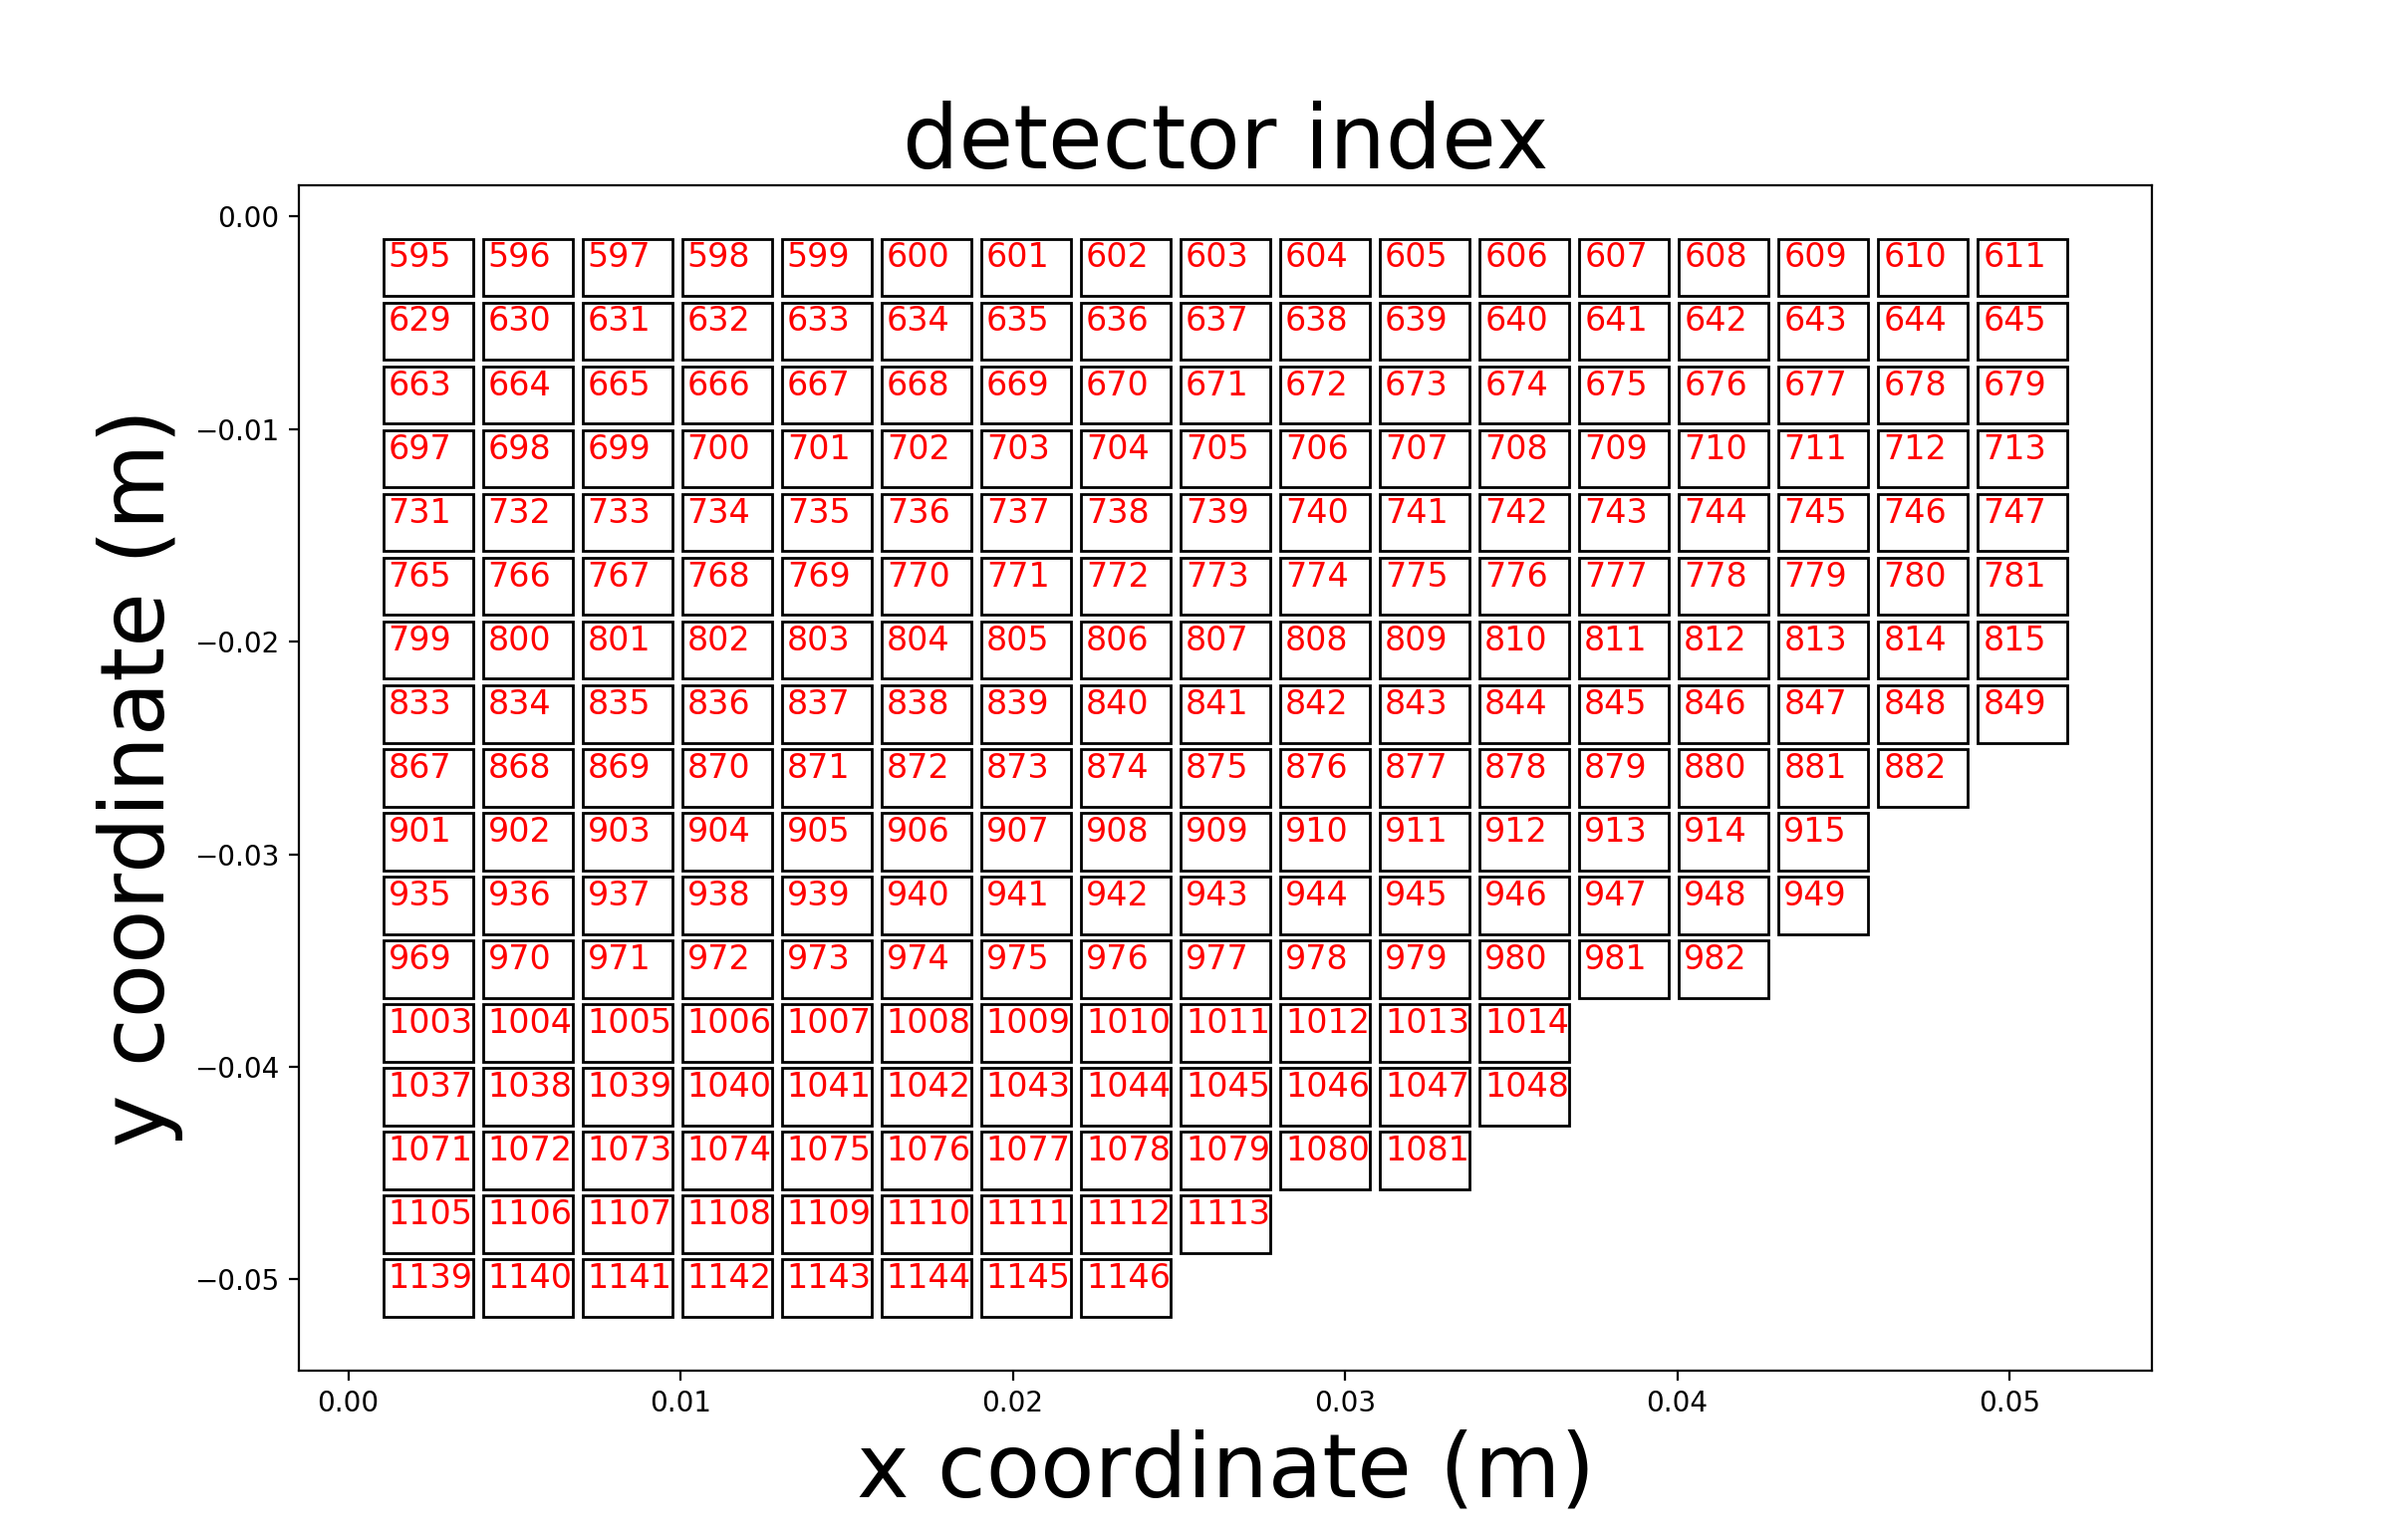
\includegraphics[width=0.6\textwidth]{det_index.png}
    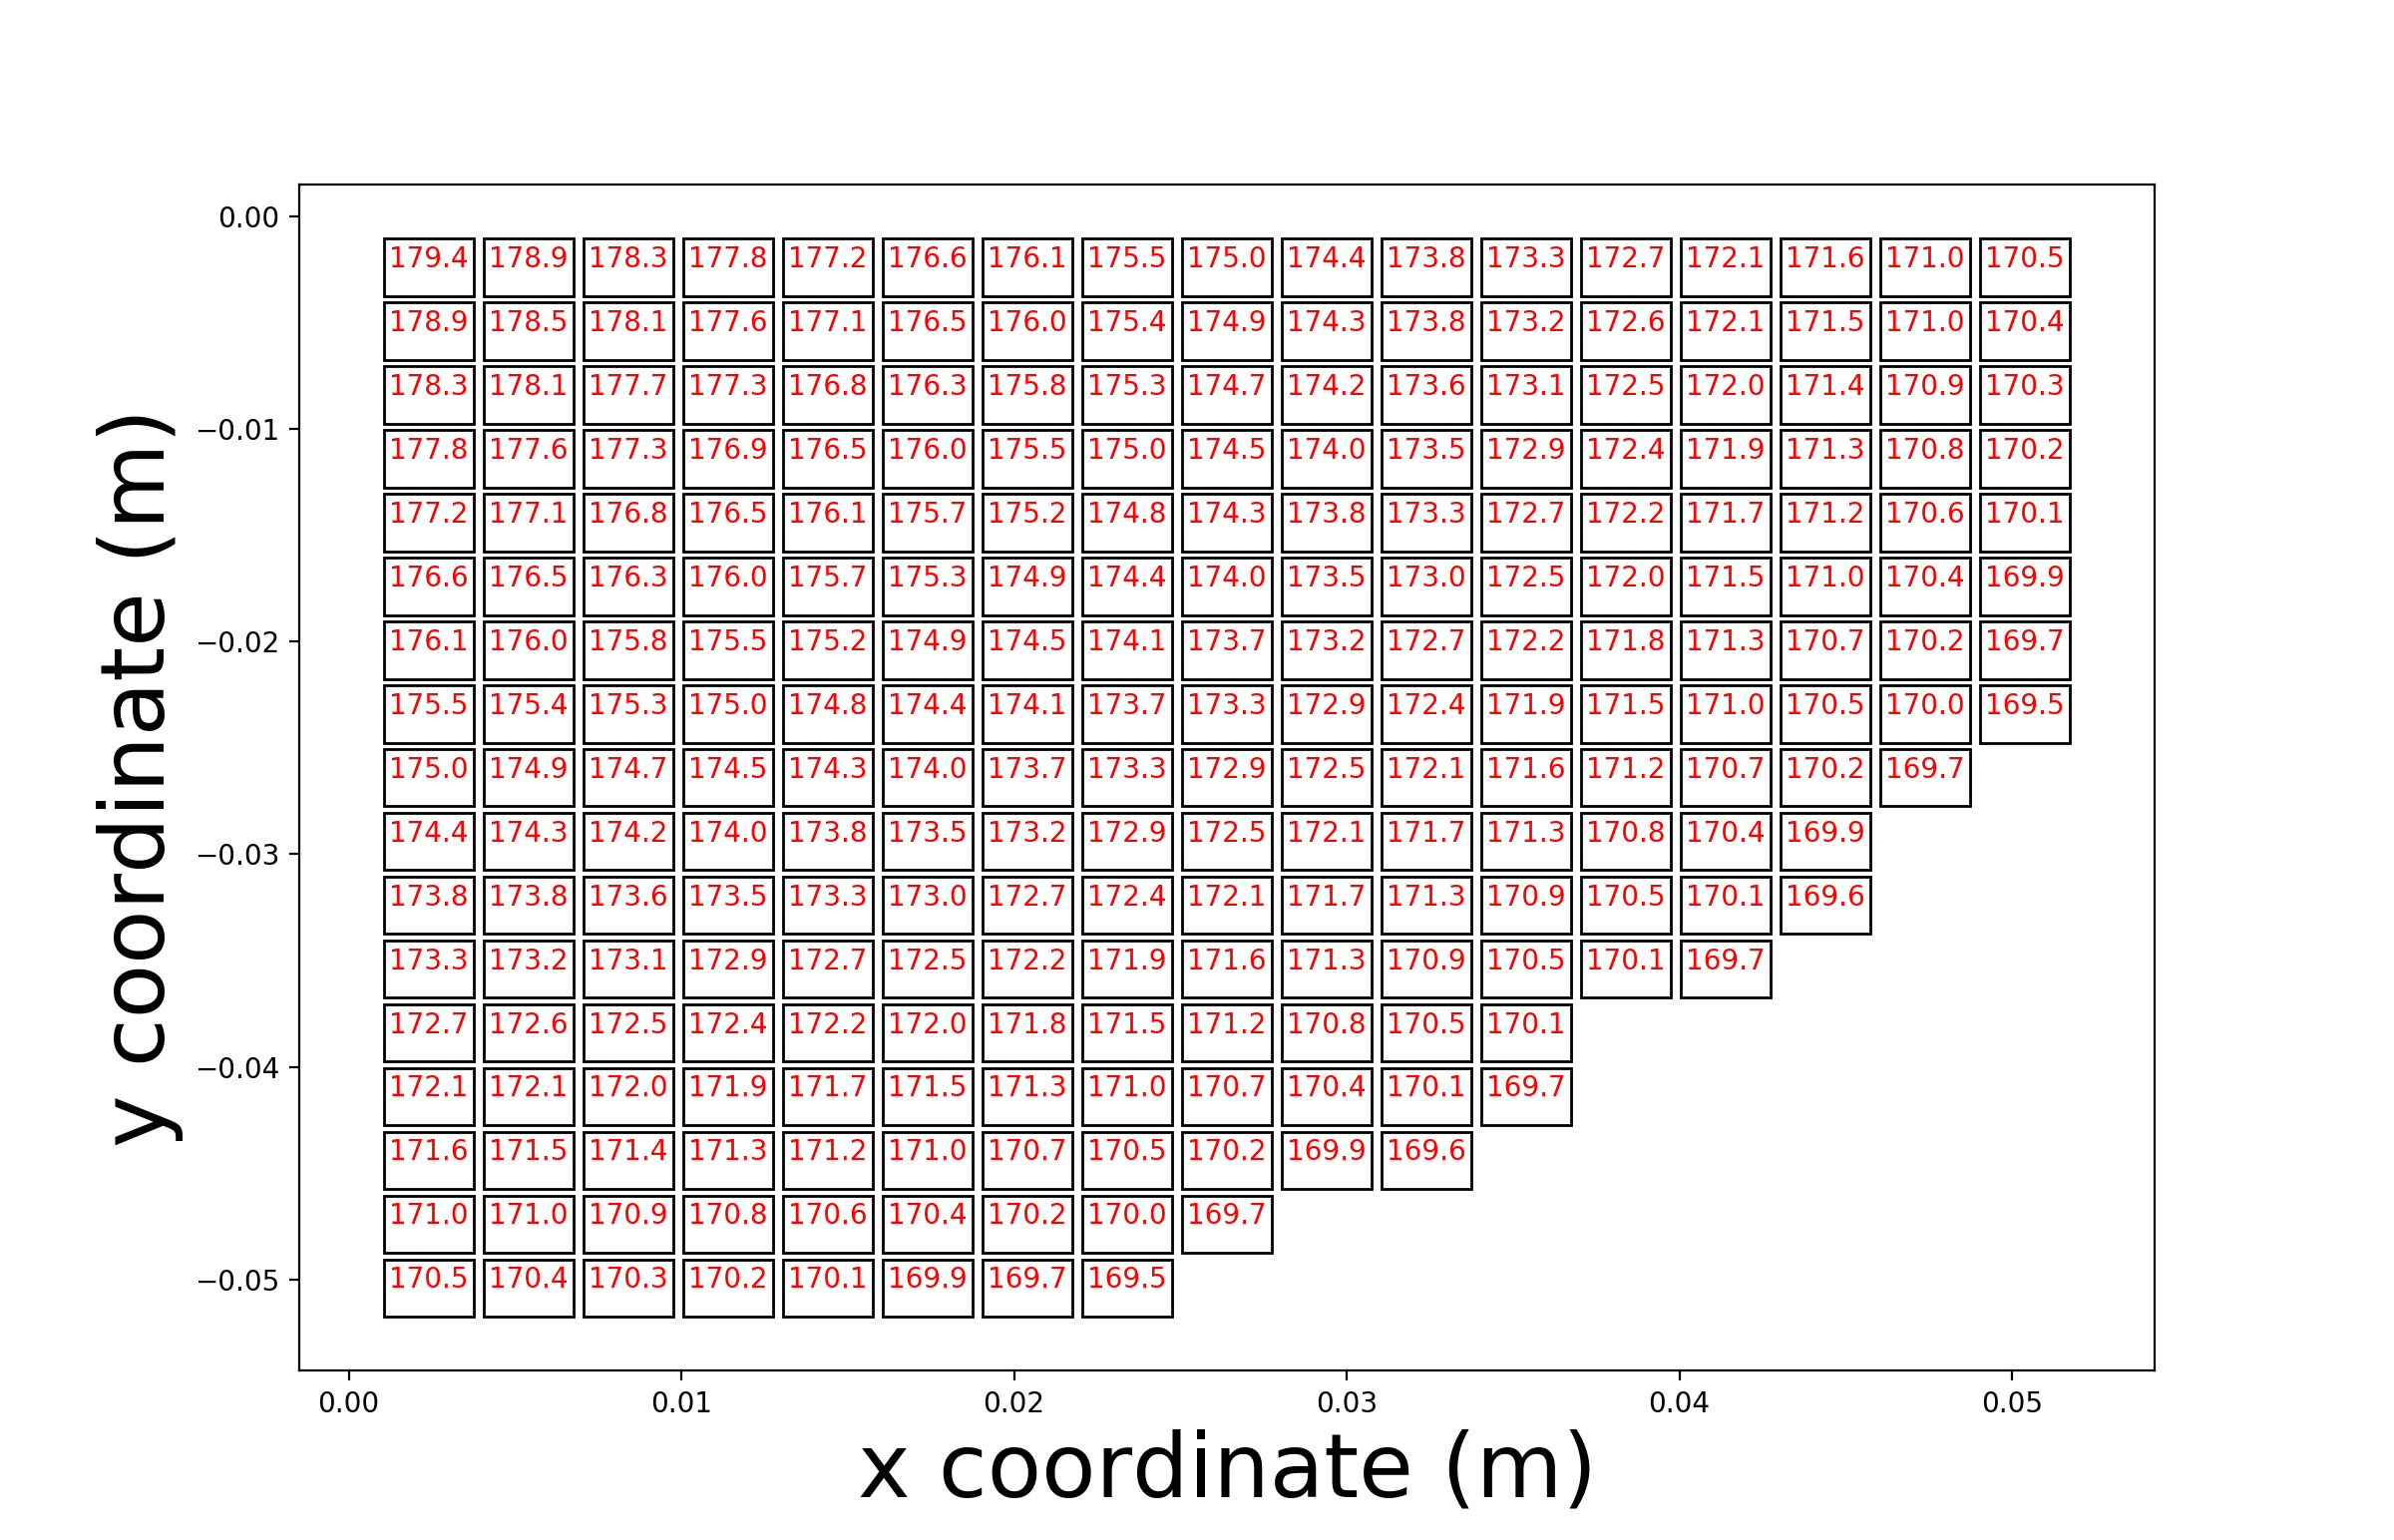
\includegraphics[width=0.6\textwidth]{theta.png}
  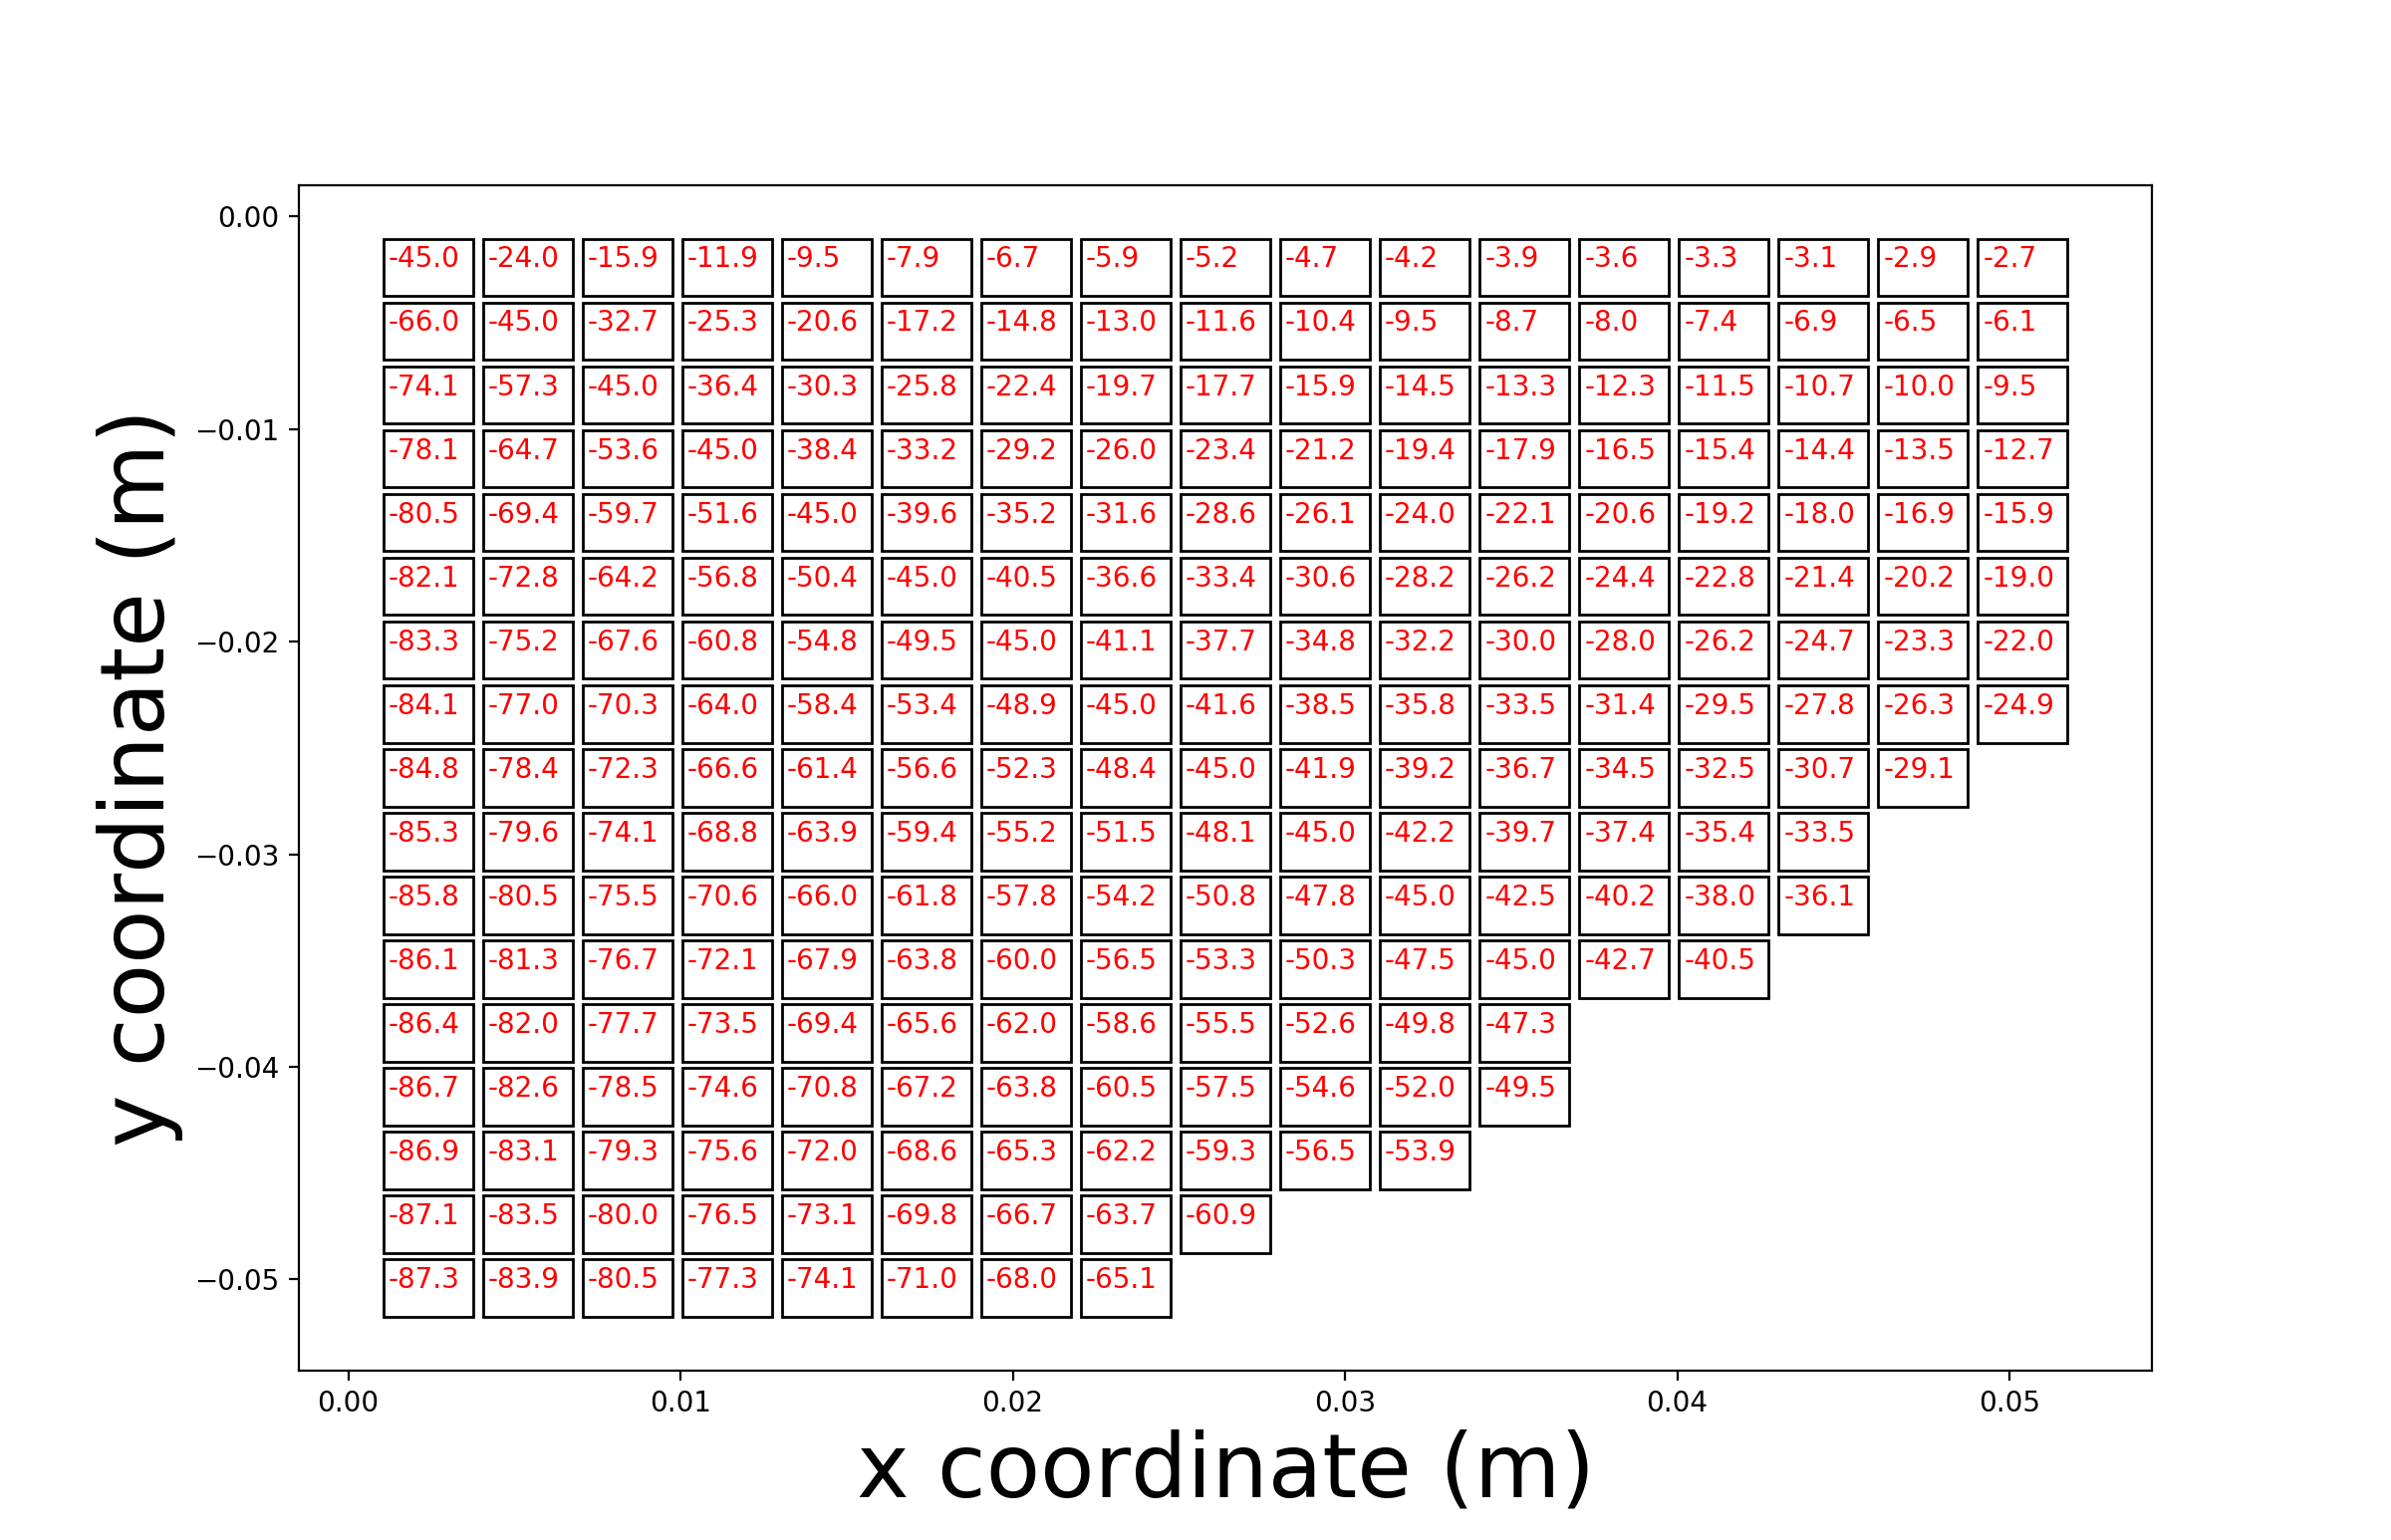
\includegraphics[width=0.6\textwidth]{phi.png}
    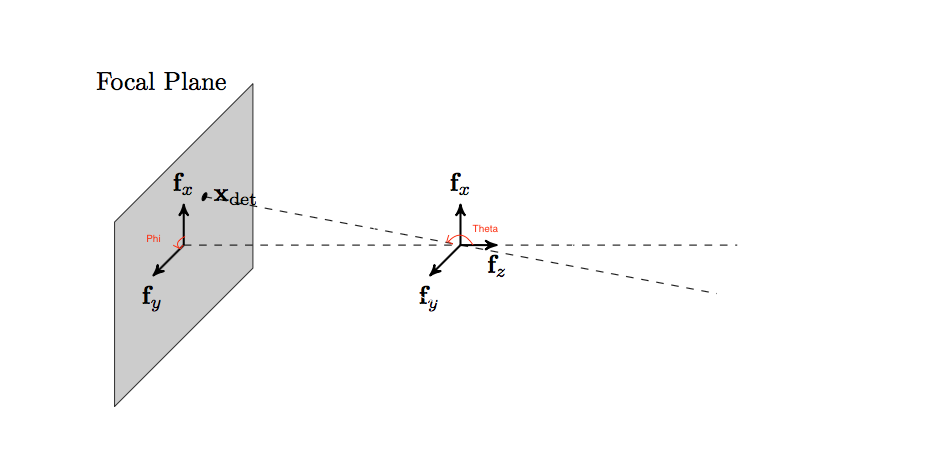
\includegraphics[width=0.6\textwidth]{focal_plane.png}
  \caption{top: detector index, middle top: $\theta$, middle bottom: $\phi$, bottom: focal plane angle .}
  \label{fig:detector_array}
\end{figure}

The layout also contain information on detectors angle, using the focal length of the telescope in the following way. It modify the coordinates array (vertex) which become a $({\rm id}^{\rm row}_{\rm det},{\rm id}^{\rm column}_{\rm det} ,4,3)$  array, the new coordinates is the focal lengh (0.3m specified in Optics) of the instrument. 
It then compute the angle of the detector on the sky in the following way
\ba
\theta &=& \arctan ( \sqrt{x^{2}+y^{2}} / f) \\
\phi &=& \arctan ( y/x )
\ea
Where x and y are the coordinates of the center of the detector.
Note that f the focal is chosen to be oriented -0.3m.

\subsubsection{ Horns array}

The horn layout is created by reading the latest version of  $\it{CalQubic\_HornArray\_v*.fits}$, we will change it in the futur to the one specify in the global.dict file.
The fits file contains the following information.
\begin{enumerate}
\item the version of the file
\item the spacing between the different horn arranged on a regular grid, the fits file contain the value 0.014 m
\item xreflection and yreflection, possible reflection around the x and y axis, set to False in the code
\item angle counter-clockwise rotation angle in degrees (45).
\item the horn radius (0.0066 m)
\end{enumerate}
This info is first read in $\it{instrument.py}$, it is then send to the Layout class.

\begin{figure}
  \centering
  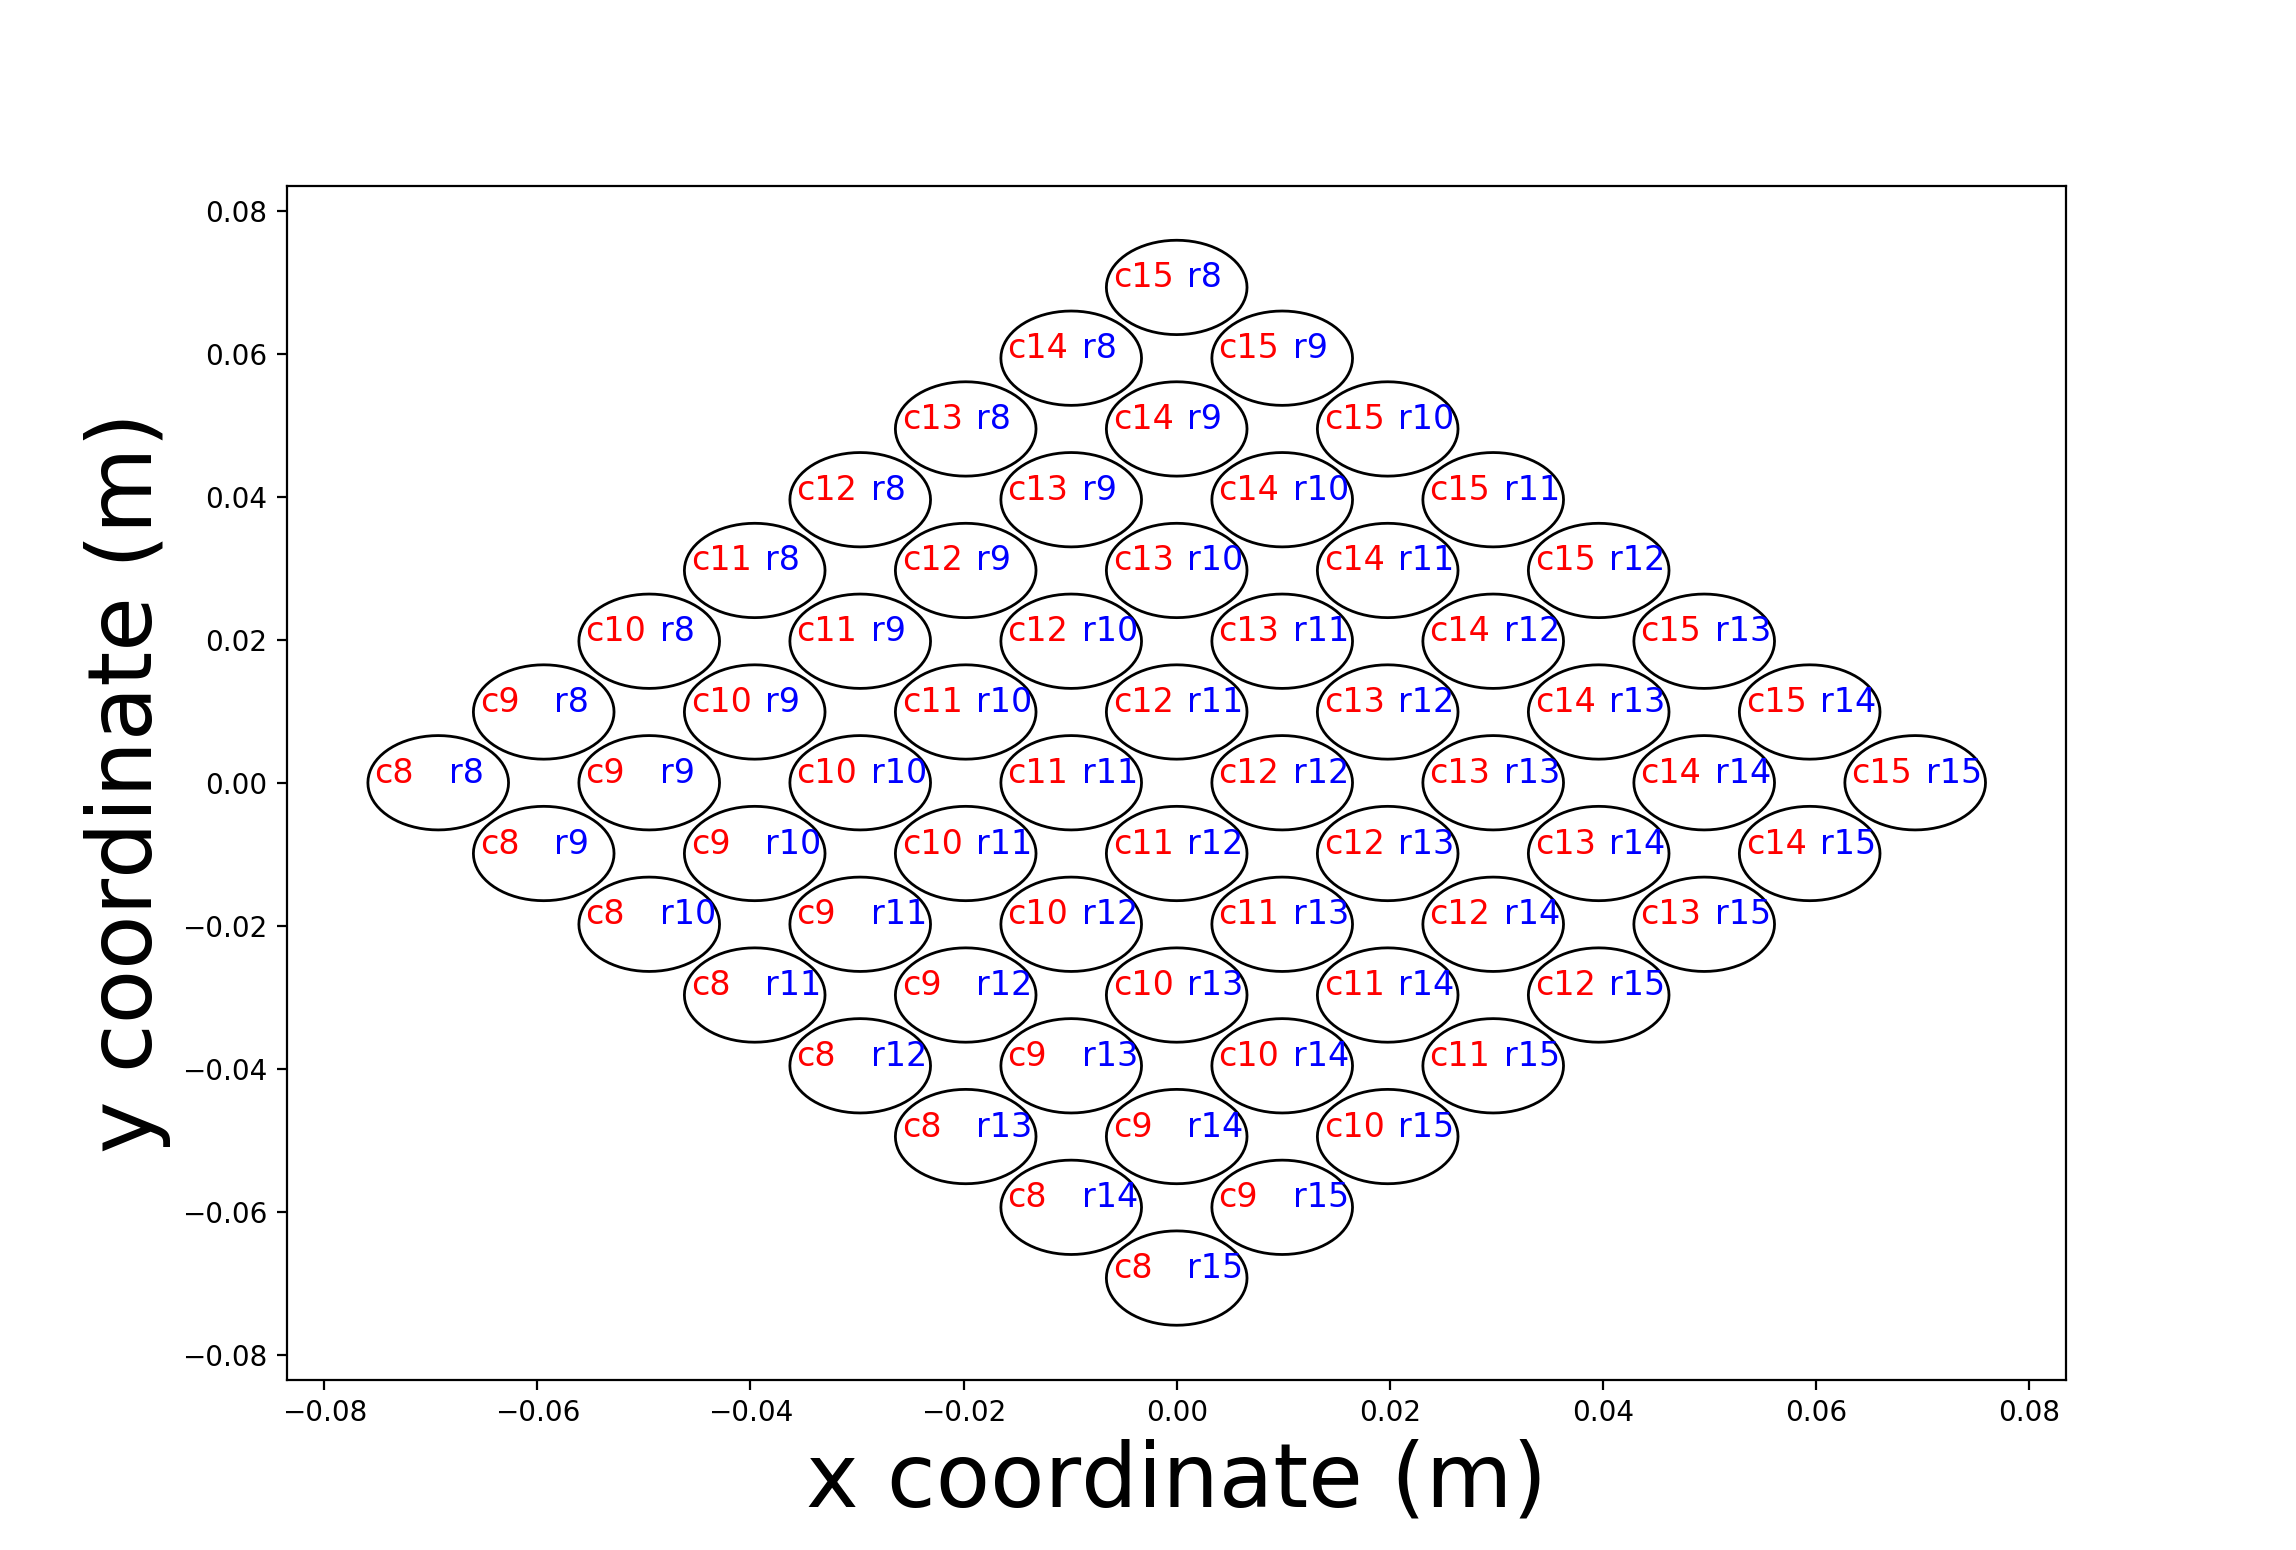
\includegraphics[width=0.6\textwidth]{hornArray.png}
  \caption{array of horn with row and column displayed}
  \label{fig:horn_array}
\end{figure}

\subsubsection{ Optics and Prim Beam}

The primary beam file $\it{CalQubic\_PrimBeam\_v*.fits}$ contains the information on the primary beam FWHM, for the instrument it is $13^{\circ}$.
The optic file $\it{CalQubic\_Optics\_v*}$ contains information about the different optical elements, namely their Temperature (K), their transmission, their emissivity and the number of polarisation state. Their are 11 optical elements listed in the file, two at 250 K (winB1 and Block2), two at 100 K (12cmEd Block3), five at 6K (8cmEd,HWP,PolGr,Ba2Ba,Combin) and two at 0.1 K (7cmEd,BandFi).

\subsection{Noise properties}

Now let's discuss a bit the way the code handles the noise.
Once you have specified an instrument (see previous subsection), you can simulate the noise seen by the different detectors. For this you have to specify a sampling (pointing) and a scene. For now on we will assume random pointing, the actual pointing will be described in details in the pointing section.
The number of detectors for the TD is 248, two source of noise affect the detector:
\begin{enumerate}
\item The detector noise
\item The photon noise
\end{enumerate}
In the following we will describe how the code handle each of these items.

\subsubsection{Detector noise}

The routine adding detector noise $\it{get\_noise\_detector}$ is called in $\it{instrument.py}$, it actually refer to the routine $\it{get\_noise}$  coded in $\it{pysimulator}$
The routine can use a PSD (power spectrum density) and the bandwidth of the instrument to generate a noise realisation.
Another usage of the routine is to specify the properties of the noise. The following properties should be used:  $ f_{\rm knee}$, $f_{\rm slope}$, ${\rm NEP}_{\rm det}$.
Remember: Noise Equivalent Power can be interpreted as the input signal
power that produces a signal-to-noise ratio of unity at the output of
a given detector at a given data-signaling rate or modulation
frequency, and effective noise bandwidth; it is the minimum
detectable power per square root bandwidth. 
\begin{enumerate}
\item If  $ f_{\rm knee}=0$, the code generate  white noise only, it first computes $\sigma=\frac{{\rm NEP}_{\rm det}}{\sqrt{2 T_s}}$, given that the NEP is in unit $W/\sqrt{\rm{Hz}}$, $\sigma$ is in Watt. $T_{s}$ is the sampling rate, set to 1 s in the code. The noise is added  in time-space.
\item if $ f_{\rm knee}\neq 0$, the noise would be added in frequency space. The psd is computed as  \\ $P(f)=\sigma^{2}(1+|f/f_{\rm knee} |^{f_{\rm slope}})/f_{s} $, then $n^{\rm det}(t)={ \cal F}^{-1}[ {\cal F}[{\cal G}^{\rm det}(0,1)(t)] \sqrt{P(f)}] \sqrt{f_{s}}$
\end{enumerate}
The noise is generated for each sample and each detector and is return as a ($n_{{\rm det}},n_{{\rm sample}}$) array

\subsubsection{Photon noise}

The photon noise represent the contribution from the loading due to the atmosphere and optic temperature. This is where the scene routine come into play.
The code takes as input the atmosphere temperature $T_{\rm atm}=200 K$, the atmosphere emissivity $\epsilon_{\rm atm}=0.015$ and the atmosphere transmission $\eta_{\rm atm}=1$, the temperature of the CMB, $T_{CMB}=2.7255 K$ as well as the temperature,  emissivity,  transmission, and polarisation states of all optical elements $T_{i}, \epsilon_{i}, \eta_{i},p_{i}=(1,2)$. The emissivity, transmission and polarisation state of the CMB are set to 1.
In the default setting of the code, there are 13 components total: (CMB, Atm +11 optics components).
Then the code compute an effective transmission for each of the component. Basically the idea is to compute the transmission of a given component on the detector array, for the CMB this transmission is given by $\eta^{\rm CMB}_{\rm eff} = \prod^{11}_{i=1} \eta_{i} $, the last component transmission between set to 1.
Then the code compute the solid angle sustained by a given detector on the sky $\Omega_{\rm det}= -\frac{A_{\rm det}}{f^{2}} \cos^{3}(\theta_{\rm det}) $ and the effective surface of the horn array $S_{\rm horn}= N_{\rm horn} \pi R^{2}_{\rm horn}$.
\begin{figure}
  \centering
  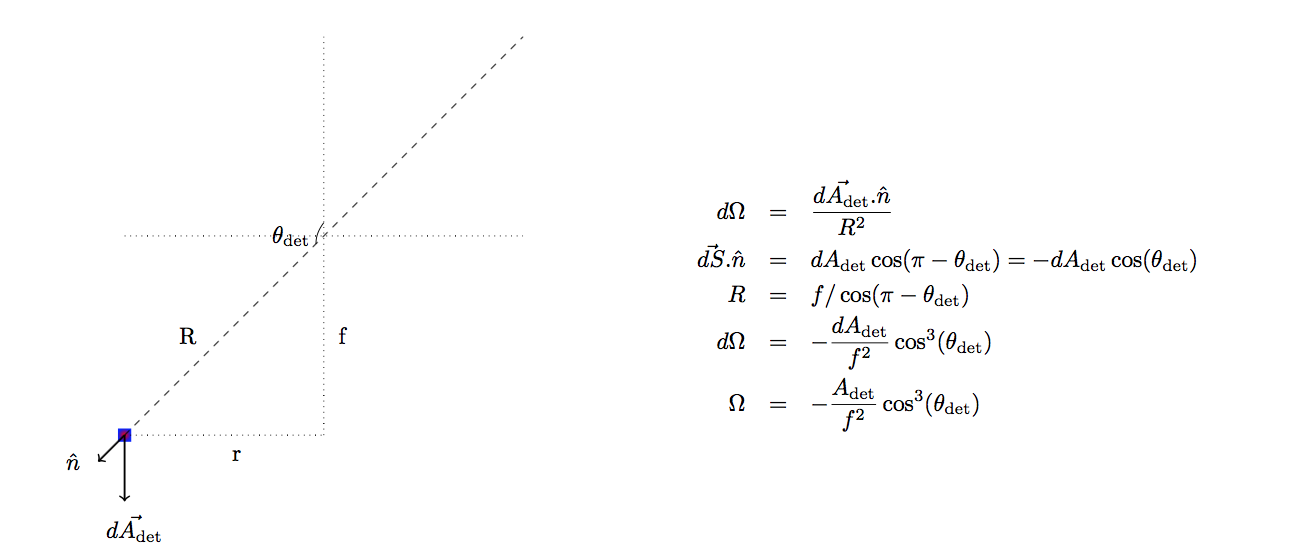
\includegraphics[width=0.8\textwidth]{solid_angle.png}
  \caption{solid angle seen by a detector on the focal plane}
  \label{fig:solid_angle}
\end{figure}

The NEP is then computed in the following way:
\ba
{\rm NEP}_{\rm \det} &=& \sqrt{ \sum_{i} 2h\nu P^{i}_{\gamma} \left(1+\frac{P^{i}_{\gamma}}{h \nu g_{i}} \right)} \\
P^{i}_{\gamma} &=& \frac{\epsilon_{i}\eta_{\rm eff,i}h\nu}{\exp (h \nu/k_{B}T_{i}) -1} g_{i} \rho_{\rm \det} B_{\rm sec}(\theta_{\rm det}) \\
g_{i} &=& p_{i} S_{\rm horn} \Omega_{\rm det} \left(\frac{\nu}{c} \right)^{2} \Delta \nu
\ea
We will need a good bibliography reference to explain this formula...
$B_{\rm sec}(\theta_{\rm det})$ is the secondary beam transmission. The secondary beam is define just like the primary beam but with the remapping $\theta=\pi-\theta$. $\rho_{\rm \det}$ is the detector efficiency, set to 0.8 in the code.
The NEP is then computed for each detector and the photon noise is added as a white noise component on the detector array.

\subsection{Time constant}

\begin{figure}
  \centering
  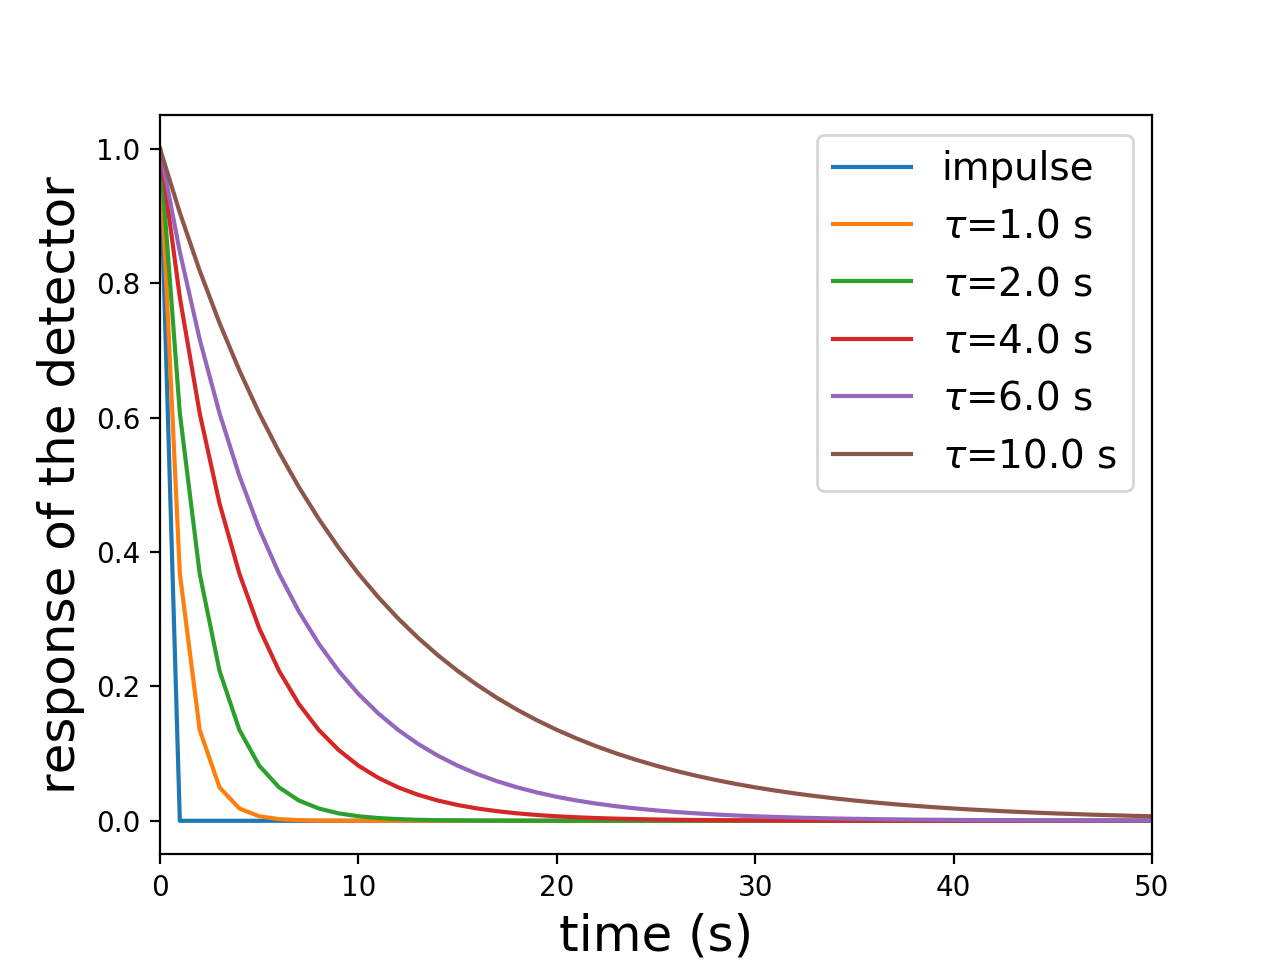
\includegraphics[width=0.8\textwidth]{time_constant.png}
  \caption{effect of the time constant on an impulse signal}
  \label{fig:time_constant}
\end{figure}

The time constant is used in $\it{get\_detector\_response\_operator}$  in $\it{instrument.py}$.
It  takes the form of an operator than can be used on a $(n_{\rm det}, n_{\rm sample})$ array.
The operator perform a convolution of the time ordered data by a truncated exponential.
The time constant appears in the following equation:
\ba
\tau \frac{d{\rm o(t)}}{dt}+ {\rm o(t)}= i(t)
\ea
Where i(t) is a source term (forcing function) and o(t) is the recovered signal. A general solution of this equation can be found using a green function
\ba
o(t)= o_0 \exp \left(-\frac{t}{\tau} \right) + \frac{1}{\tau} \int^{t}_{0^{+}} i(t') \exp \left( -\frac{(t-t')}{\tau} \right) dt'
\ea
Or more simply in Fourier space
\ba
\tilde{o}(\omega)=\tilde{i}(\omega) \frac{ 1-i\omega t }{ 1+ (i\omega t)^{2}}
\ea

In the code, this convolution is done efficiently using the following difference equation
\ba
o_{n}=(1- \exp(-\frac{1}{f_{s}\tau})) i_{n}  + \exp(-\frac{1}{f_{s}\tau})o_{n-1}
\ea 
Where $f_{s}$ is the sampling frequency $f_{s}=1/T_{s}$ and $T_{s}$ is set to 1s by default in the code.
The time constant convolution is coded up as an operator in the code. The action of the operator is coded up in $\it{pysimulators}$, in the fortran routines  $\it{operators.f90.src}$ and $\it{module\_operators.f90.src}$. We illustrate the effect of time constant on a impulse at t=0 in Figure \ref{fig:time_constant}. 

\subsection{Beam}

They are three relevant beam for QUBIC, the primary beam, the secondary beam and the synthetic beam.
\subsubsection{Primary and secondary beam}

The primary beam and secondary beam are defined as un-normalized Gaussian with  $ \sigma_{\rm FWHM}=13^{\circ}$
\ba
B_{\rm prim}(\theta, \phi)&=& \exp( - \frac{\theta^{2}}{2 \sigma^{2}})  \\
B_{\rm sec}(\theta, \phi)&=& \exp( - \frac{ (\pi -\theta)^{2}}{2 \sigma^{2}})  \\
 \sigma &=& \sigma_{\rm FWHM} / \sqrt{8\log 2}
\ea
They are returned as healpix map in the code, a figure showing the healpix map as well as the projection on the north (primary) and south (secondary) spherical cap is displayed in Figure \ref{fig:prim_second_beam}
\begin{figure}
  \centering
  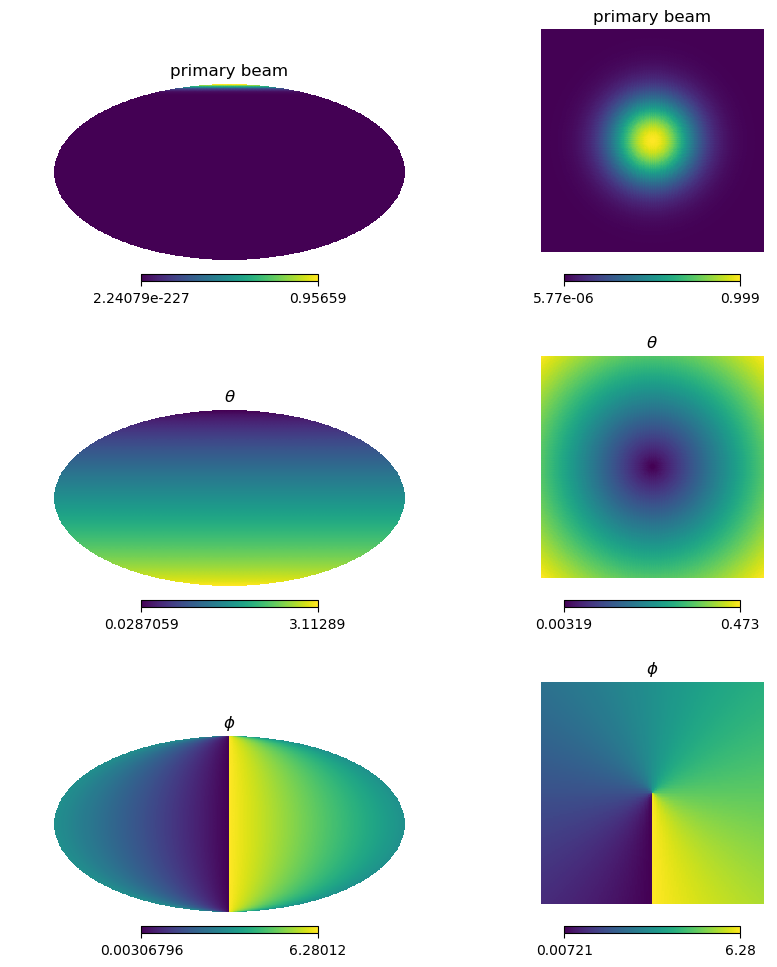
\includegraphics[width=0.4\textwidth]{primary_beam.png}
    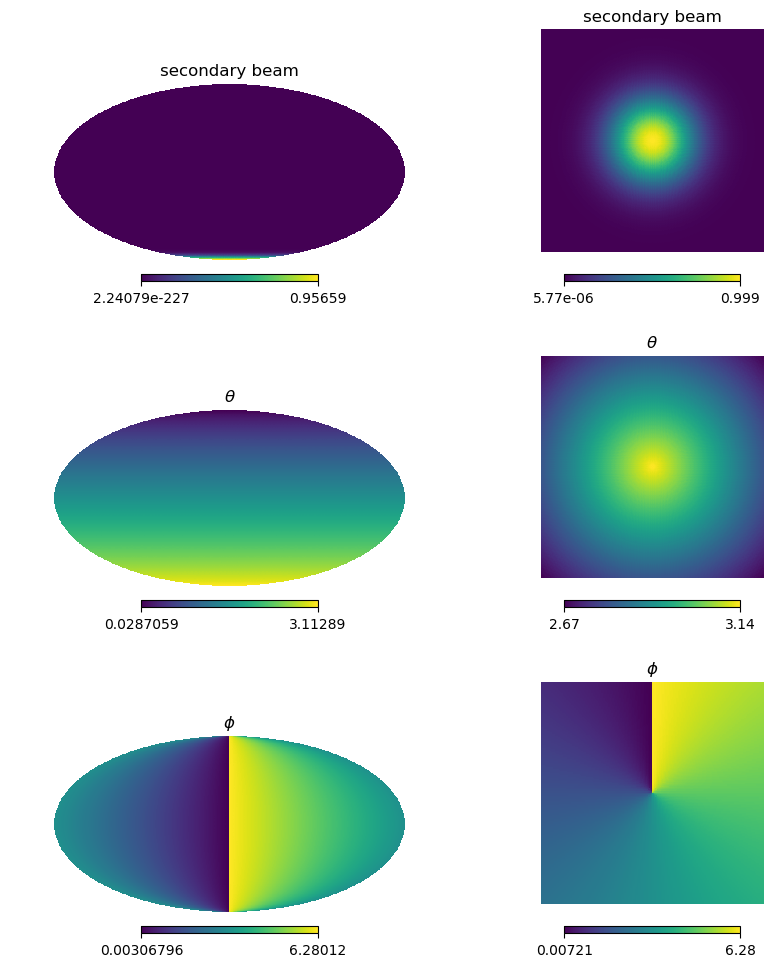
\includegraphics[width=0.4\textwidth]{secondary_beam.png}
  \caption{primary and secondary beam respectively projected on the north and south spherical cap}
  \label{fig:prim_second_beam}
\end{figure}

\subsubsection{Synthetic beam}




The computation of the synthetic beam is more subtle as it involves the diffraction by the horn arrays and is computed for each detector on the focal plane.
It can be obtained using the $\it{get\_synthbeam}$ routine in $\it{instrument.py}$. The routine takes as argument a scene (which is basically only used to specify the resolution of the healpix map to display the synthetic beam), an index for the detector for which we want to compute the synthetic beam (if not specified, the beam is returned as an ($n_{\rm det}$, $n_{\rm pix}$) array where  $n_{\rm pix}$ is the number of pixel of the healpix map, and $\theta_{\rm max}$, the maximum zenithal angle above which the synthetic beam is assumed to be zero. The code then call the static method $\it{\_get\_synthbeam}$ still in $\it{instrument.py}$ with argument scene, the position of the detector (3d coordinate ($x_{c},y_{c},z_{c}$) in m where $z_{c}$ is the  focal lenght), the area of the detector ($m^{2}$), $\nu$, $\Delta \nu$, the horn array specifications, the primary and secondary beam and the data type of the synthetic beam (float32 by default).
The code then compute the healpix $\theta$ and $\phi$ array corresponding to the $n_{\rm side}$ of the healpix map and call the routine $\it{\_get\_response}$. \\

One subtlety happen during this call, the bandwidth  $\Delta \nu= 37.5$ GHz is called as a spectral irradiance. Note that the primary function of $\it{\_get\_response}$ is to return the monochromatic complex field $\sqrt{(W/ {\rm Hz})}^{1/2}$ related to the electric field over a specified area of the focal plane created by sources of specified spectral irradiance $W/(m^{2}.{\rm Hz} )$ . In the code the sky (created by scene) is assumed to be in $W/(m^{2}.{\rm Hz} )$, by passing the bandwidth, I believe the code assume that the sky is integrated along the bandwidth (but it's a bit weird) and that the beam size is independent of frequencies (weird again). \\

There are two different effect we need to consider the first one is the light incident on the horn array, then the transmission between the back of the horn array to the detector array.

\begin{enumerate}
\item The complex electric amplitude and phase going through each horn can be computed as 
\ba
E^h(\theta,\phi)&=& E^h_{0}(\theta,\phi) \exp ( \frac{2 i \pi \nu} {c} \vec{x}_{\rm horn}. \hat{n})  \\
 E^h_{0}(\theta,\phi)&=& \sqrt{ \Delta_{\nu} B_{\rm prim}(\theta, \phi) \pi r^{2}_{\rm horn} }
\ea
Here $\vec{x}_{\rm horn}$ is a 3d vector with cartesian coordinates $(x_{\rm horn},y_{\rm horn},z_{\rm horn}=0)$ and \\ $\hat{n}=(\sin \theta \cos \phi, \sin \theta \sin \phi, \cos \theta)$ is the spherical radial unit vector in cartesian coordinates.
The result is given as a $(n_{\rm horn}, n_{\rm pix})$ array.
\item The Phase and transmission from the switches to the detectors on the focal plane
\ba
T^{h}_{\rm det} (\theta_{\rm det}, \phi_{\rm det}) &=&T^{h}_{0, { \rm det} }(\theta_{\rm det}, \phi_{\rm det}) \exp ( \frac{2 i \pi \nu} {c} \hat{x}_{\rm det}. \vec{x}_{\rm horn}) \\
&=& \sqrt{  B_{\rm sec}(\theta_{\rm det}, \phi_{\rm det}) \frac{\Omega_{\rm det}}{\Omega_{\rm sec} }}
\ea
Here $\Omega_{\rm det}$ is the solid angle sustain by the detector, $\Omega_{\rm sec}$ is the solid angle of the secondary beam. $\hat{x}_{\rm det}$ is a cartesian unit vector pointing toward the detector  (with $z_{\rm det}=-f$)
$T^{h}_{\rm det}$ is a $(n_{\rm det}, n_{\rm horn})$ array. The code use $\it{ne.evaluate}$ for the fast evaluation of array expressions elementwise.
\end{enumerate}
\begin{figure}
  \centering
  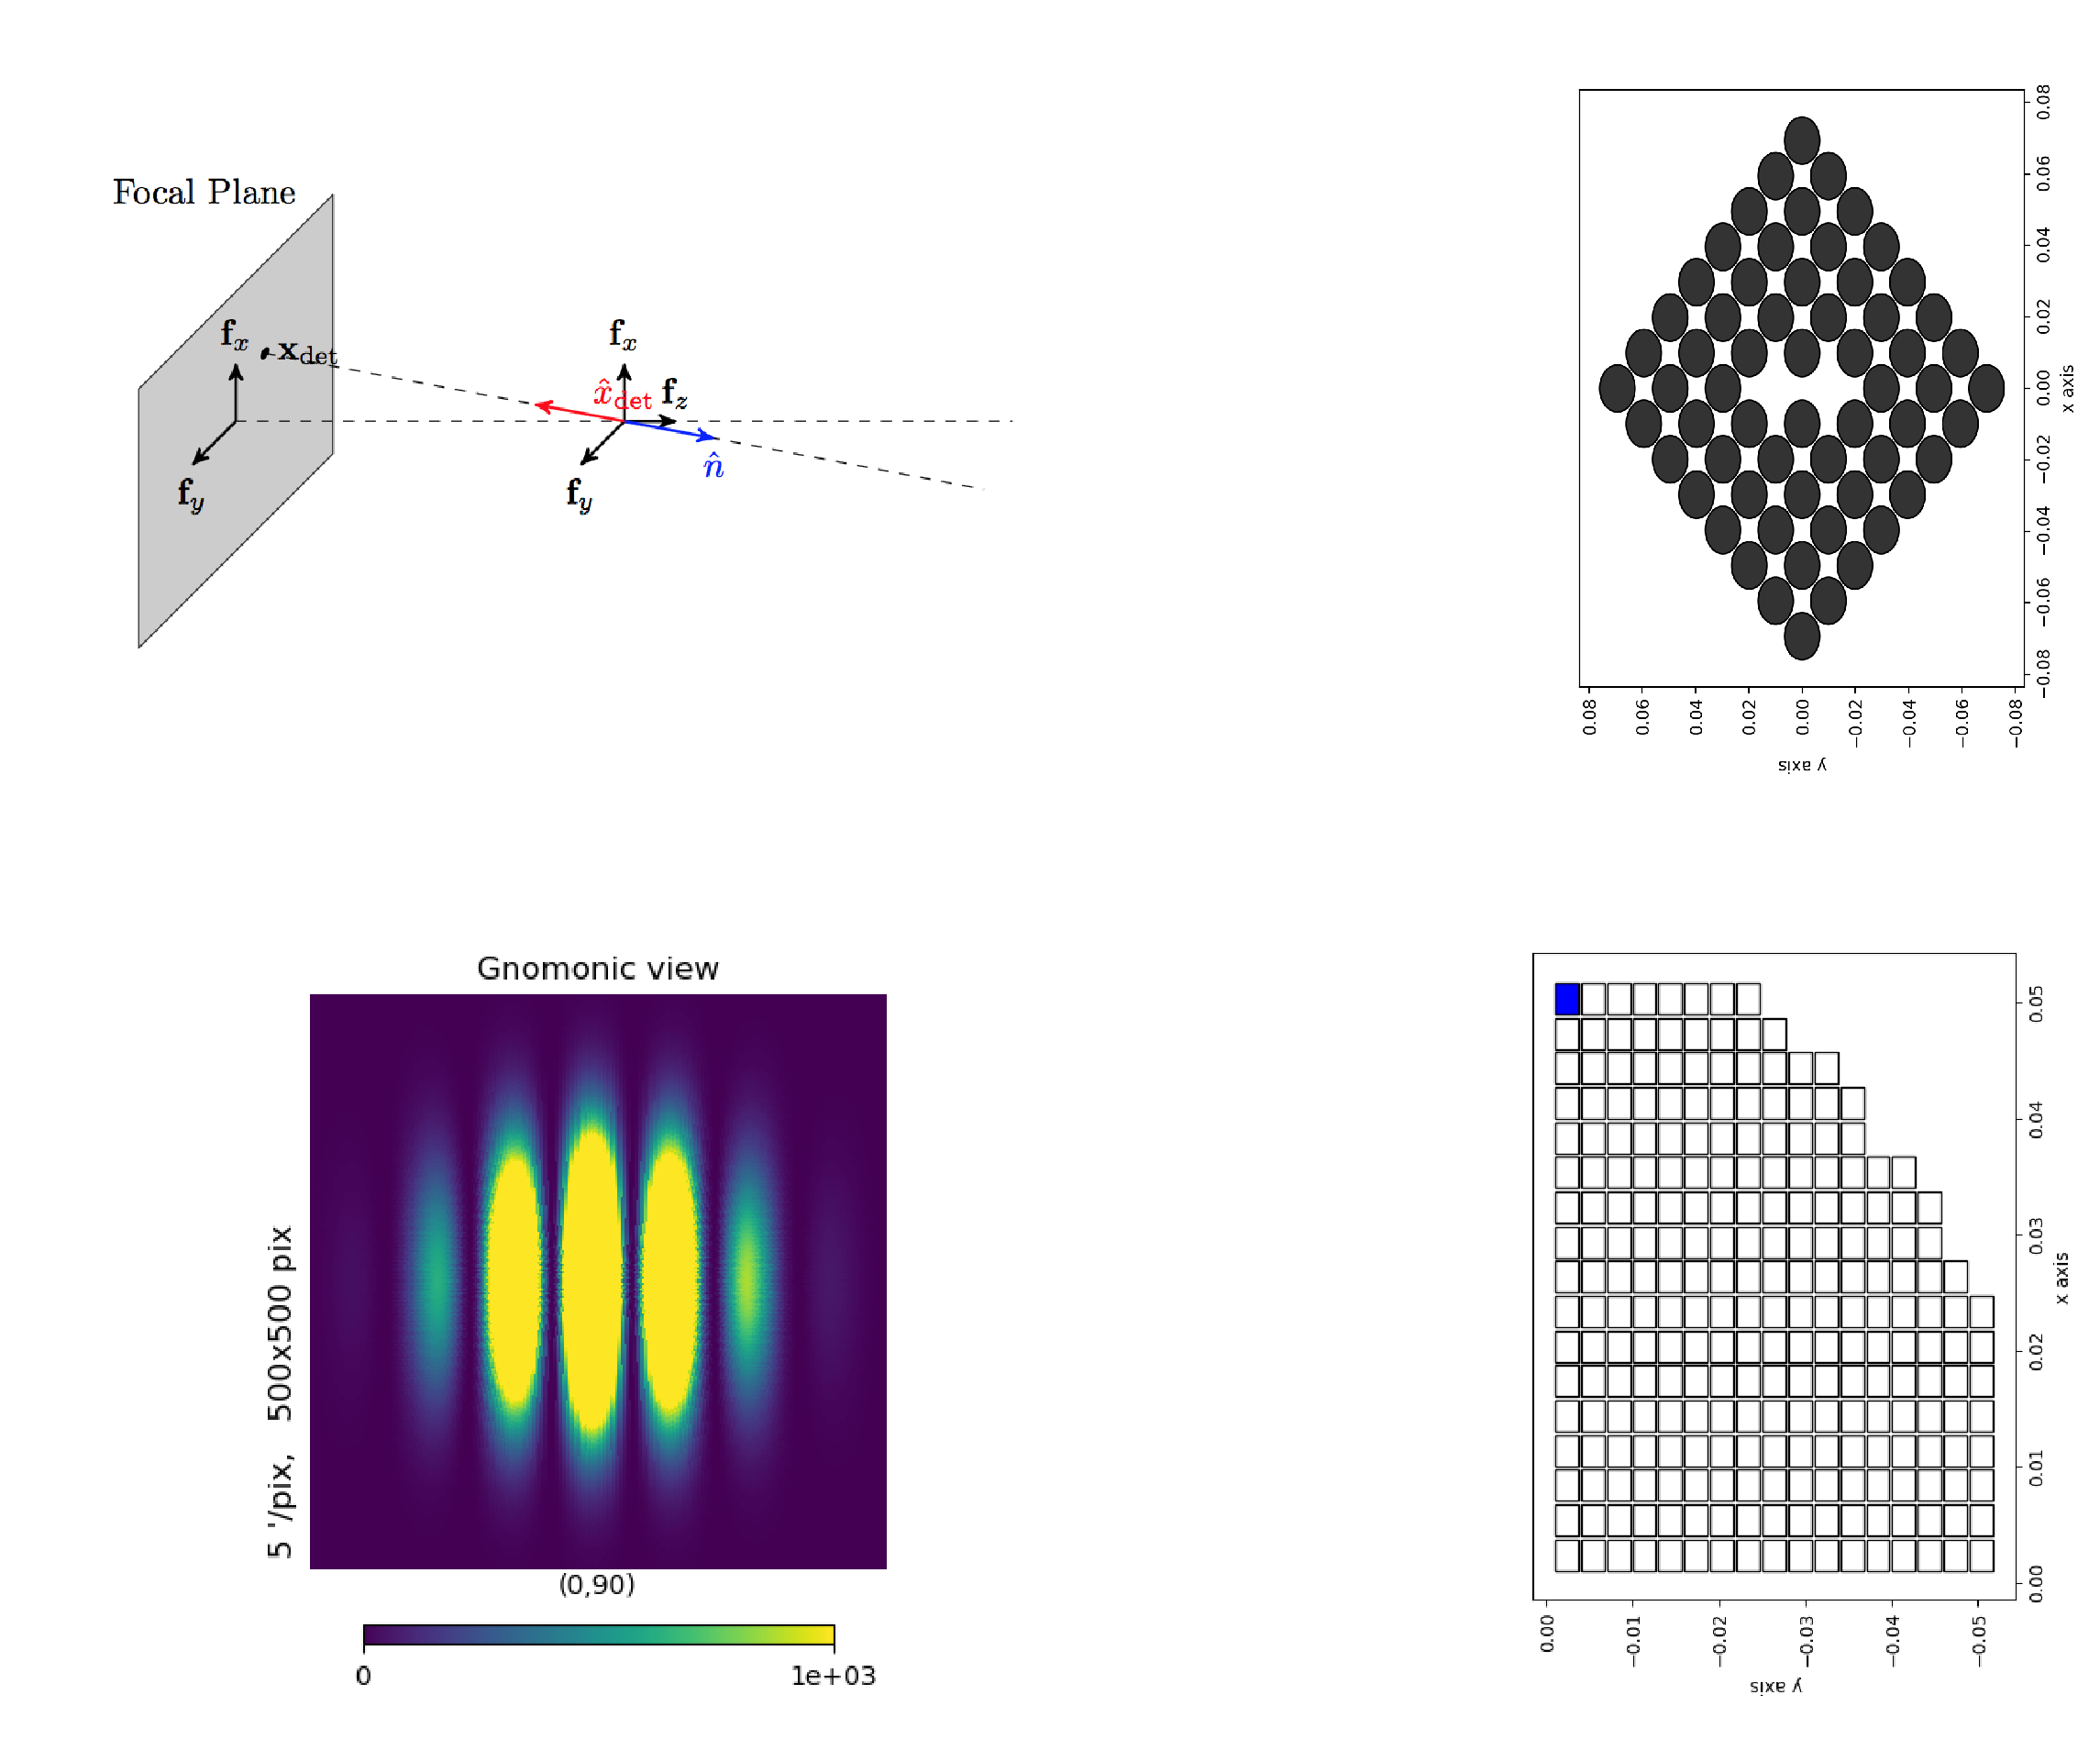
\includegraphics[width=0.8\textwidth]{synthetic_beam_2horn_open_000.png}
  \caption{synthetic beam for two horns open}
  \label{fig:prim_second_beam}
\end{figure}

The synthetic beam is then returned as
\ba
B^{\rm synth}_{\rm det}(\hat{n})= \Delta_{\nu} B_{\rm prim}(\theta, \phi) \pi r^{2}_{\rm horn}  B_{\rm sec}(\theta_{\rm det}, \phi_{\rm det}) \frac{\Omega_{\rm det}}{\Omega_{\rm sec} } \bigg| \sum^{N_{h}}_{h=1} \exp \left( \frac{2 i \pi \nu} {c}   \vec{x}_{\rm h} ( \hat{x}_{\rm det} + \hat{n} ) \right) \bigg|^{2}
\ea
We can comment a bit on the last term which source the interference pattern, let's define $i \vec{\alpha}= \frac{2 i \pi \nu} {c}  ( \hat{x}_{\rm det} + \hat{n} ) $, for two horns open (j and k) we have
\ba
( e^{i \vec{\alpha}. \vec{x}_{j}}+e^{i \vec{\alpha}. \vec{x}_{k}}   ) ( e^{-i \vec{\alpha}. \vec{x}_{j}}+e^{-i \vec{\alpha}. \vec{x}_{k}}   ) = 2(1+ \cos (\vec{\alpha}.(\vec{x}_{j}-\vec{x}_{k})))
\ea
Now let's try to compute this term when we have all horns open except two. For doing this let's first compute the interference pattern when all horns are open
\ba
S_{\rm tot} =\bigg| \sum^{N_{h}}_{h=1}  e^{ i \alpha \vec{x}_{\rm h}} \bigg|^{2} = N_{h} +\sum^{N_{h}}_{j=1}  \sum_{k \neq j}\cos (\vec{\alpha}.(\vec{x}_{j}-\vec{x}_{k}))
\ea
The expression for all horns open but the horn i is:
\ba
S_{-i} = S_{\rm tot} -1 - \sum_{k \neq i} 2 \cos (\vec{\alpha}.(\vec{x}_{i}-\vec{x}_{k}))
\ea
The expression for all horns open but the horns i and j is
\ba
S_{-ij} &=& S_{\rm tot} -2 - \sum_{k \neq i} 2 \cos (\vec{\alpha}.(\vec{x}_{i}-\vec{x}_{k}))- \sum_{k \neq  j} 2 \cos (\vec{\alpha}.(\vec{x}_{j}-\vec{x}_{k})) + 2 \cos (\vec{\alpha}.(\vec{x}_{j}-\vec{x}_{i})) \\ 
S_{-ij} &=& S_{-i} + S_{-j} + 2 \cos (\vec{\alpha}.(\vec{x}_{j}-\vec{x}_{i})) - S_{tot}
\ea
Note that this expression differs from the one presented in the self-calib paper, they are aware that they have a typo.


\subsection{Multifrequencies}

The code also allow for constructing a multiband instrument. The first step  is to specify a number of frequencies subband $\nu$, this is done in the code with the routine $\it{compute\_ freq}$ in  $\it{polyacquisition.py}$.
The code take an input frequency say $\nu=150 {\rm GHz}$, a relative band width $\frac{\delta \nu}{\nu}=0.25 $ and the number of frequencies we want to cut this band into $N_{\rm freq}=10$. The code start by computing $\nu_{\rm min}=\nu(1-\frac{\delta \nu}{\nu})$ and $\nu_{\rm max}(1+\frac{\delta \nu}{\nu})$, and use interpolation in log space to define a set of sub-bands between them.

The output of the code are
\ba
N_{\nu, {\rm edges}} &=& N_{\nu}+1  \text{ The  number of frequency edges} \\
\nu_{\rm edges} && \text{ The  location of the edges} \\
\nu  && \text{ The center frequency of each sub-band} \\
\delta  && \text{ The size of each sub-band} \\
\Delta  && \text{ The size of the full band} \\
N_{\nu}  && \text{ The number of frequencies of the sub-band}
\ea

Note that this routine is used both for simulating the instrument (at the moment this is arbitrary and is chosen to be 10) and for recovering the final product as a function of output frequencies.




\section{Pointing}

They are two different pointing method implemented in the code, they can be found in $\it{samplings.py}$. One of them is realistic: $\it{create\_sweeping\_pointings}$ and one of them allow for fast test of the code $\it{create\_random\_pointings}$
Both methods return the azimuth (A), the elevation (h), the pitch angle ($\gamma$) and the hwp angle  ($\eta$)  for each sample.
For both pointing methods you start by specifying the center of the patch in equatorial coordinate (${\rm{RA_c}}$ ,${\rm{DEC_c}}$).
For both methods, the HWP angle is computed as
\ba
\eta(t)=11.25 {\cal I}(0,7)(t)
\ea
where ${\cal I}(0,7)$ represent integer random number between 0 and 7.

\subsection{Random Ponting}

For random pointing, you have to specify the number of sample you want, this is done with the argument $n_{\rm pointings}$, you also have to specify the maximum angular distance to the center of the patch $d\theta$. Optional arguments are the date of observation ($T_{0}$ default being '2016-01-01 00:00:00'), the observer latitude and longitude (default is DOME C: lat = -(75 + 6 / 60)  long = 123 + 20 / 60).
The code start by generating $n_{\rm pointings}$ random number for $\theta$, $\phi$ and $\gamma$ in the following way 
\ba
\theta(t) &=& \arccos ( \cos d\theta + (1- \cos d\theta ){\cal U}_{0}(0,1)(t) ) \\
\phi(t) &=& 2\pi {\cal U}_{1}(0,1)(t)  \\
\gamma(t) &=& 2\pi {\cal U}_{2}(0,1) (t)
\ea
Where ${\cal U}_{n}(0,1)$ are random number uniformly distributed between 0 and 1.
It then compute the time at which is sample is taken: $t_{i}= T_{0}+  i \delta t$, note that default is $\delta t=1$s in the code.
Finally it use a set of operators:
 \begin{enumerate}
\item Cartesian2SphericalOperator (${\cal O}_{c \rightarrow s} $)  :  (see $\it{pyoperators/nonlinear.py }$) \\ Convert cartesian unit vectors into spherical coordinates, The spherical coordinate system is defined by: \\
  - the zenith direction of coordinate (0, 0, 1) \\
  - the azimuthal reference of coordinate (1, 0, 0) \\
 - the azimuth signedness: it is counted positively from the X axis  to the Y axis. \\
 Four conventions define what the two spherical angles are \\
- 'zenith, azimuth':  angles commonly used in physics or the (colatitude, longitude) angles used in the celestial and geographical coordinate systems \\
- 'azimuth, zenith': (longitude, colatitude) convention \\
- 'elevation, azimuth: (latitude, longitude) convention \\
 - 'azimuth, elevation': (longitude, latitude) convention  
\item CartesianEquatorial2HorizontalOperator (${\cal R}_{e \rightarrow h} $): (see $\it{pysimulators/operators.py}$)  \\   Conversion between equatorial-to-horizontal cartesian coordinates. \\
The ICRS equatorial direct referential is defined by: \\
 - the Earth center as the origin \\
 - the vernal equinox of coordinates (1, 0, 0) \\
- the Earth North pole of coordinates (0, 0, 1) \\
 The horizontal referential is defined by: \\
 - the observer geographic position as the origin \\
 - the azimuth reference (North or South) of coordinates (1, 0, 0) \\
 - whether the azimuth is measured towards the East or West \\
 - the zenith of coordinates (0, 0, 1)

\item Rotation3dOperator  (${\cal R}_{\rm rot})$: (see $\it{pyoperators/linear.py }$) \\
Operator for 3-d active rotations about 1, 2 or 3 axes. \\
The rotation axes are specified one by one by selecting a convention. \\
For intrinsic rotations (in which the coordinate system changes with the rotation), the following conventions are possible: \\
X, Y, Z, \\
 XY', XZ', YX', YZ', ZX', ZY', \\
 XZ'X'', XZ'Y'', XY'X'', XY'Z'',  YX'Y'', YX'Z'', \\
YZ'Y'', YZ'X'', ZY'Z'', ZY'X'', ZX'Z'' and ZX'Y''. \\
The primes denote the rotated axes after the first elemental rotation and the double primes the rotated axes after the second one. \\
And for the extrinsic rotations (in which the original coordinate system remains motionless): \\
 X, Y, Z, \\
XY, XZ, YX, YZ, ZX, ZY,  \\
 XZX, XZY, XYX, XYZ, YXY, YXZ, YZY, YZX, ZYZ, ZYX, ZXZ and ZXY. 
\item Spherical2CartesianOperator  (${\cal O}_{s \rightarrow c} $):  (see $\it{pyoperators/nonlinear.py }$) \\
 Convert spherical coordinates into  cartesian unit vectors 
\end{enumerate}
The full rotation to get azimuth and elevation from $\theta$ and $\phi$ is then 
\ba
A(t),h(t)=   {\cal O}^{\rm az,el}_{c \rightarrow s} ({\cal R}^{\rm NE}_{e \rightarrow h} (t) ({\cal R}^{\rm Z  Y'}_{\rm rot} [ {\rm RA_{c}, 90- DEC_{c} }] ({\cal O}^{\rm zen, az}_{s \rightarrow c} (\theta(t),\phi (t)))))
\ea


\subsection{Sweeping Pointing}
As for the random pointing, you start by specifying the center of the patch in equatorial coordinate (${\rm{RA_c}}$ ,${\rm{DEC_c}}$).
Then you compute the azimuth and elevation corresponding to the center of the patch as a function of time (given the starting date of observation, the sampling period and the observer latitude and longitude). 
\ba
A_{c}(t), h_{c}(t)=  {\cal R}^{\rm NE}_{e \rightarrow h} (t) ({\rm{RA_c}} ,{\rm{DEC_c}})
\ea
Where ${\cal R}^{\rm NE}_{h \rightarrow e} (t)$ is the SphericalEquatorial2HorizontalOperator (see $\it{sampling.py/equ2hor}$).
For the sweeping pointing routine, we have to specify the duration of the observation $t_{\rm obs}$, in hours, the number of samples is then given by $n_{\rm pointings}=\frac{3600 t_{\rm obs}}{T_{s}}$ with $T_{s}$ the sampling period.
We also have to specify the azimuth extent of a scan  $\Delta A$, and the angular speed $\omega$ of the scan. The time it takes to scan back and forth is then given by $t_{bf}= \frac{2 \Delta A}{\omega}$. The sweeping index is then trivially given by $i_{\rm sweep}(t)= \left \lfloor{\frac{t}{t_{bf}}}\right \rfloor $, the azimuth offset for each sample is  given by
\ba
\epsilon (t)&=& \omega t  \ ({\rm mod} \ 2\Delta A ) \\
\tilde{\epsilon} (t)&=&
  \begin{cases}
    \epsilon (t) & \text{if  $\epsilon (t)< \Delta A$} \\
    -\epsilon (t) +2\Delta A  & \text{otherwise}
  \end{cases} \\
\delta A(t)&=& -\frac{\Delta A}{2}+ \tilde{\epsilon} (t) \\
\ea
For the elevation, you also have to specify the number of sweep at constant elevation  $n^{h}_{\rm sweep}$. The elevation index is given by $i^{h}_{\rm sweep}(t)=\frac{i_{\rm sweep}(t)}{n^{h}_{\rm sweep}}$ which is used to specify h(t).
Finally we have
\ba
A(t)&=& A_{c}(t)+\delta A(t) \\
h(t)&=& h(i^{h}_{\rm sweep}(t))
\ea
Finally the pitch angle is computed using a pitch velocity $\omega_{\gamma}$ (default 0.1 degree/s) and a maximum pitch angle $\gamma_{\rm max}$ (default 10 degree)
\ba
\epsilon_{\gamma} (t)&=& \omega_{\gamma} t  \ ({\rm mod} \ 4\gamma_{\rm max} ) \\
\tilde{\epsilon_{\gamma}} (t)&=&
  \begin{cases}
    \epsilon_{\gamma} (t) & \text{if  $\epsilon_{\gamma} (t)< 2\gamma_{\rm max}$} \\
    -\epsilon_{\gamma} (t) +4\gamma_{\rm max}& \text{otherwise}
  \end{cases} \\
\gamma(t)&=& -\gamma_{\rm max}+ \tilde{\epsilon}_{\gamma} (t) \\
\ea
I have also added an option in my version of the code for doing scan of a fixed source.

\begin{figure}
  \centering
  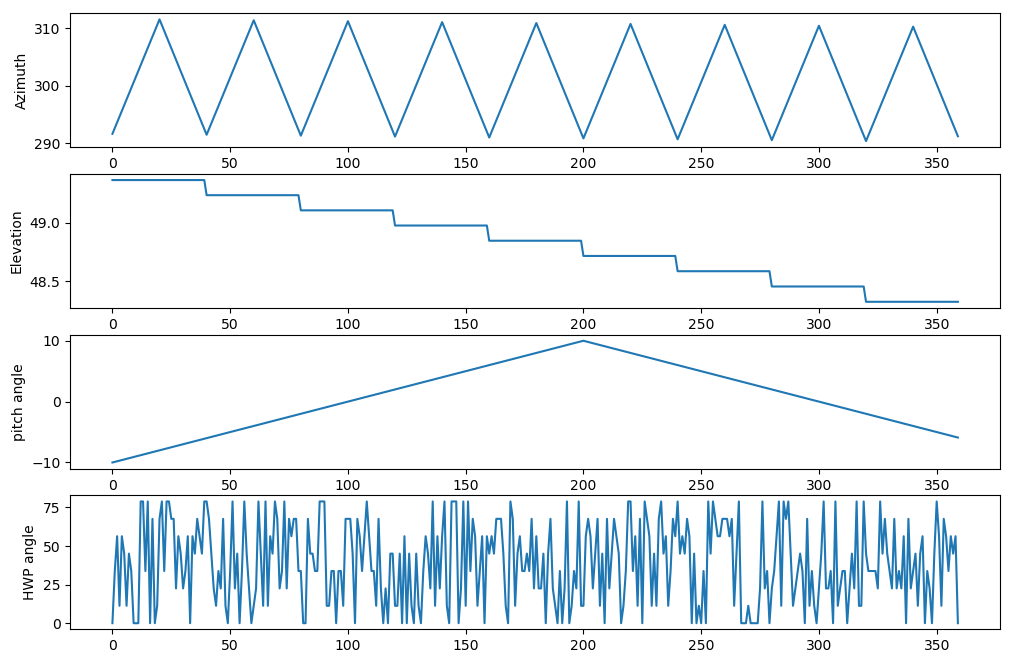
\includegraphics[width=1\textwidth]{sweeping_pointing.png}
  \caption{6 minutes sweeping scan from La Puna, the center of the patch is chosen at RA=0, DEC=0}
  \label{fig:prim_second_beam}
\end{figure}



\section{Acquisition}

For a multifrequencies instrument, they are two different acquisition methods. The polyacquisition method and the multiacquisition method. 
The multiacquisition method being simply a generalisation where we get observation for different frequencies subbands.

\subsection{Multiacquisition}

The main function in the the $\it{multiacquisition.py}$ routine is the $\it{get\_observation}$ function.
It takes an array of maps of the form ($N_{\rm sub}$, $n_{\rm pix}$, $n_{\rm stokes}$) where $N_{\rm sub}$ is the number of frequencies sub-bands, $n_{\rm pix}=12 N^{2}_{\rm side} $ and $n_{\rm stokes}$ is the number of Stokes parameter ($n_{\rm stokes}=3$ for I,Q,U), and create a TOD for each detector (TOD being the detector signal as function of time). The function has two optional argument, convolution and noiseless.
If noiseless=False, no noise will be added to the TOD. In the following I will describe what convolution do and how we go from a map to a TOD.

\subsubsection{Convolution}

The default value for convolution is convolution=TRUE, the convolution is done using the \\ $\it{get\_convolution\_peak\_operator}$ defined in $\it{instrument.py}$.
This routine depends on the argument ripples, if ripples=True the operator is  $\it{ConvolutionRippledGaussianOperator}$ which takes as argument the frequency of the subbands. Otherwise the convolution is done with the $\it{HealpixConvolutionGaussianOperator}$, with  $\sigma_{\rm fwhm}(\nu^{i})= \sigma^{150}_{\rm fwhm} \frac{150 . 10^{9}}{ \nu^{i}}$
The later is simply done in pixel space with the healpy smoothing function, while the former is done in $\it{ripples.py}$ in harmonic space.
The default value in the code is ripples =False, For now we will not describe the ripple convolution in details as I don't think it's extremely relevant for the rest of the analysis.
The result is a convolved map for each of the sub-bands, and it is from this set of map that we will generate the TOD.

\subsubsection{From map to TOD}

This subsubsection could be a section by itself as it is truly the core of the code, how to take a healpix map and project it to a TOD.
The main function is $\it{get\_operator}$ in $\it{acquisition.py}$, it creates the H operator which consist of the composition of many different operators
\ba
{\cal H}=  {\cal R}_{\rm det}  {\cal T}_{\rm inst}   {\cal I}_{\rm det}  {\cal P}_{\rm ol} [{\cal H}_{\rm WP} * {\cal P}_{\rm roj}]  {\cal F}_{\rm ilt}  {\cal A}_{\rm p}  {\cal T}_{\rm atm}  {\cal U}_{\rm nit}   {\cal D}_{\rm ist}
\ea 
The TOD is then obtained by the operation ${\rm TOD}= {\cal H}(m)$ where m is the map.
In the following, we will describe what does each of these operators.

\begin{enumerate}
\item  ${\cal D}_{\rm ist}$ is a MPI operator. It distributes a global map, of which each MPI process has a copy, to the MPI processes. It is a block column operator whose blocks are identities distributed across the MPI processes.
\item The ${\cal U}_{\rm nit} $ operator convert sky temperature into $W / m^2 / {\rm Hz}$, the conversion applied to healpix pixel is 
\ba
{\cal U}_{\rm nit}= \frac{10^{-6}}{T} \frac{2\Omega_{pix}h \nu^{3}}{c^{2}} \frac{h \nu}{k T} \frac{e^{ \frac{h \nu}{k T}}}{(e^{ \frac{h \nu}{k T}}-1)^{2}}
\ea
the operator can be found in  $\it{pysimulators/interfaces/healpy/scenes.py}$
\item ${\cal T}_{\rm atm}$ is the atmosphere transmission, it is set to 1 by default in the code
\item ${\cal A}_{\rm p} $ is the aperture integration operator, it integrates flux density in the telescope aperture, this convert signal from $W / m^2 / Hz$ into $W / Hz$. It is coded in $\it{instrument.py}$. It is an homothety (a rescaling by a scalar) of value $\lambda= N_{\rm horn} S_{\rm horn}= N_{\rm horn} \pi r^{2}_{\rm horn}$ 
\item ${\cal F}_{\rm ilt}$ is the filter operator, it converts units from W/Hz to W, it is again an homothety operator with $\lambda=\delta \nu$ (the bandwidth)
\item $ {\cal P}_{\rm roj}$ is the projection operator, converting  W to W/sr, the core of the code $\it{\_get\_projection\_operator}$ is in $\it{instrument.py}$. It takes as argument a rotation, the scene, the central frequency $\nu$, the position (center location of the detectors), the synthetic beam, the horn and the primary beam. This operator takes a $(n_{\rm pix},n_{\rm stokes})$ map and return a $(n_{\rm det},n_{\rm sample}, n_{\rm stokes})$ TOD. An example of such TOD can be found in Figure \ref{fig:TOD}. So how does this work?

The first step is to compute the spherical coordinates ($\theta^{\rm det}_{i}$, $\phi^{\rm det}_{i}$) of the beam peaks for each detector, in radians, up to a maximum diffraction order,  with the routine ${\it \_peak\_angles}$ in  ${\it instrument.py}$.
The diffraction order is used to decide which the peaks are ignored. For instance, a value of $k_{\rm max}=2$ will model the synthetic beam by $(2  k_{\rm max} + 1)^{2} = 25$ peaks and a value of $k_{\rm max}=0 $ will only sample the central peak.
This is done by computing a normed position vector for each detector in the focal plane $\hat{x}^{\rm det}= \frac{ \bm{x^{det}}}{ |\bm{x^{det}}|}$, then the code define a mesh Fourier grid $\bm{k}$ with $k_{x}$ and $k_{y}$ $\in [-k_{\rm max}, k_{\rm max}]$ ($k_{\rm max}$ is set to 8 by default in the code), the location of the peaks is then found as $n^{\rm det}_{i,x}= \hat{x}^{\rm det}_{x} - \frac{c}{\nu} \frac{k_{i,x}}{d_{h}}$ where $d_{h}$ is the horn spacing and similar for $n_{y}$.
 Finally 
\ba
\theta_{i}^{\rm det} &=&\arcsin \sqrt{( n^{\rm det}_{i,x})^{2} + (n^{\rm det}_{i,y})^{2} } \\
\phi_{i}^{\rm det}&=&\arctan \frac{n^{\rm det}_{i,y} }{n^{\rm det}_{i,x}} 
\ea
This only tells you that the peaks of the synthesized beam are separated by an integer times  $\lambda/ d_{h}$, while this is sound, we can test if this is the case for the technical demonstrator which has an inhomogeneous horn distribution.
After doing the test, we realized there was a mismatch between the inferred beam peak position and the actual beam peak position. This was due to the rotation of 45 degree of the horn array which was not properly propagated in the ${\it \_peak\_angles\_kmax}$ routine. This is now fixed we have an argument to rotate the mesh grid  $k_{x}$ and $k_{y}$. For $k_{max}=8$, the default value in the code, the number of peaks is 289 however, most of them can not be represented in the code (they give nan in the  $\arcsin$ routine as the argument takes value $>1$) . At the end, only 14 values of $\theta$ and $\phi$ are selected. The code also compute an integration factor at each peak position
\ba
A_{i}^{\rm det}= \frac{ B(\theta_{i}^{\rm det} , \phi_{i}^{\rm det}) \Omega^{150}_{\rm beam} (\frac{150}{\nu})^{2}}{\Omega_{\rm pix}} N_{h}
\ea
Then the code create an array of the form $\hat{n}^{\rm  det}_{\rm peak}$  of shape $(n_{\rm det}, n_{\rm peak}, 2)$ where $\hat{n}_{\rm peak}^{\rm det}$= ($\theta^{\rm det}_{\rm peak}$, $\phi^{\rm det}_{\rm peak}$)  and change coordinate from the spherical frame to a cartesian frame using the $\it{Spherical2CartesianOperator}$, the resulting array is of the form $\hat{x}_{\rm peak}^{\rm  det}$  of shape $(n_{\rm det}, n_{\rm peak}, 3)$ where $\hat{x}_{\rm peak}^{\rm  det}$ is the usual normed position vector at the peaks position.
For each detector (the parallelization is on the number of detector), a change of coordinate is applied, namely the transpose of ${\it cartesian\_galactic2instrument}$  (${\cal R}_{g \rightarrow i} $) . 
\ba
{\cal R}_{g \rightarrow i} (t) =    {\cal R}^{\rm Z  Y' Z"}_{\rm rot} [ {\rm az}, {\rm 90-el },  {\rm pitch}]  {\cal R}^{NE}_{e \rightarrow h}(t) {\cal R}_{g \rightarrow e}
\ea
The position vector in the new coordinates is:
\ba
\hat{x}^{\rm gal, det}_{\rm peak} (t) =  [{\cal R}_{g \rightarrow i}]^{T} (t) \hat{x}_{\rm peak}^{\rm  det} 
\ea
corresponding to the synthetized beam peaks position of each detectors as a function of time. The resulting product is a series of $n_{\rm det}$ array of shape$ (n_{\rm sample}, n_{\rm peak}, 3) $ 
We then use the cartesian to healpix operator ${\cal O}_{c \rightarrow h}$, to associate an healpix pixel to the the synthetized beam peaks position 
\ba
 \#^{\rm gal, det}_{\rm peak} (t) =  {\cal O}_{c \rightarrow h} \hat{x}^{\rm gal, det}_{\rm peak} (t)
\ea
$ \#^{\rm gal, det}_{\rm peak} (t)  $ being a $ (n_{\rm sample}, n_{\rm peak}, 3) $ array which can be used to identify the relevant healpix pixel .
Now, that we have identified the healpix pixels corresponding to the synthetized beam peaks position of each detectors as a function of time, we will also need to rotate the polarisation.

We define $\hat{e}_{\theta}$, $\hat{e}_{\phi}$, the unit vectors defining the plane orthogonal to the pointing vector $\hat{x}_{\rm peak}^{\rm  det}$ in the frame of the instrument.
In spherical  coordinates we have
\ba
\hat{x}^{\rm  det}_{\rm peak} = \begin{bmatrix} \sin \theta \cos \phi \\  \sin \theta \sin \phi  \\ \cos \theta \end{bmatrix}
\hat{e}^{\rm  det}_{\theta} = \begin{bmatrix}   \cos \theta \cos \phi \\  \cos \theta \sin \phi  \\ -\sin \theta \end{bmatrix}
\hat{e}^{\rm  det}_{\phi}=  \begin{bmatrix} - \sin \phi \\ \cos \phi \\ 0 \end{bmatrix}
\ea
Which becomes, in cartesian coordinates
\ba
\hat{x}^{\rm det}_{\rm peak} = \begin{bmatrix}x\\y \\z \end{bmatrix}
\hat{e}^{\rm  det}_{\theta} = \begin{bmatrix}xz/\sqrt{1-z^{2}} \\yz/\sqrt{1-z^{2}} \\- \sqrt{1-z^{2}} \end{bmatrix}
\hat{e}^{\rm  det}_{\phi}=  \begin{bmatrix} -y/\sqrt{1-z^{2}} \\ x/\sqrt{1-z^{2}} \\ 0 \end{bmatrix}
\ea
We then change frame and now compute the pointing vector as given in the galactic frame
\ba
\hat{x}^{\rm gal, det}_{\rm peak} (t) =  [{\cal R}_{g \rightarrow i}]^{T} (t) \hat{x}_{\rm peak}^{\rm  det} 
\ea
We then define a new plane orthogonal to the pointing vector in galactic coordinate, in this plane we will have
\ba
\hat{e}^{\rm gal, det}_{\phi}=  \begin{bmatrix} -y^{\rm gal}/\sqrt{1-(z^{ \rm gal })^{2}} \\ x^{\rm gal}/\sqrt{1-(z^{ \rm gal })^{2} } \\ 0 \end{bmatrix}
\ea
This vector can then be rotated back in the plane of the instrument
\ba
\hat{e}^{\rm  det}_{\phi, \rm rot} =   [{\cal R}_{g \rightarrow i}] (t) \hat{e}^{\rm gal, det}_{\phi} 
\ea
The rotation of the plane can then be expressed using the scalar product of the rotated vector with the initial vector
\ba
\cos \alpha &=&   \hat{e}^{\rm  det}_{\phi, \rm rot} . \hat{e}^{\rm  det}_{\phi} \\
\sin \alpha &=&   \hat{e}^{\rm  det}_{\phi, \rm rot} . \hat{e}^{\rm  det}_{\theta}
\ea
This is then assigned to a {\it FSRRotation3dMatrix} (see {\it pysimulators/sparse}), with element $(11:A , 22 : A \cos 2 \alpha , 23:  -A \sin 2 \alpha)$ the action of this operator on a vector being
\ba
\begin{bmatrix}  I_{\rm out}  \\ Q_{\rm out} \\ U_{\rm out} \end{bmatrix}  &=& M \begin{bmatrix}   I_{\rm in}  \\ Q_{\rm in} \\ U_{\rm in} \end{bmatrix}
\ea
\ba
M^{\rm  det}_{\rm peak}(t) &=&
\begin{pmatrix} 
A^{\rm  det}_{\rm peak}(t) & 
0 & 
0 & 
\cr
0 & 
A^{\rm  det}_{\rm peak}(t) \cos 2 \alpha^{\rm  det}_{\rm peak}(t) & 
A^{\rm  det}_{\rm peak}(t) \sin 2 \alpha^{\rm  det}_{\rm peak}(t)  & 
  \cr
0 & 
-A^{\rm  det}_{\rm peak}(t) \sin 2 \alpha^{\rm  det}_{\rm peak}(t) & 
A^{\rm  det}_{\rm peak}(t) \cos 2 \alpha^{\rm  det}_{\rm peak}(t) & 
\cr
\end{pmatrix}
\ea
Overall we have a $(n_{\rm det}, n_{\rm time}, n_{\rm stokes}) \times (n_{\rm pix},  n_{\rm stokes})$ Projection operator whose action can be summarized as
\ba
\begin{bmatrix}  I^{\rm det}(t)  \\ Q^{\rm det}(t) \\ U^{\rm det}(t) \end{bmatrix}  &=&  \sum_{\rm peak} M^{\rm  det}_{\rm peak}(t)  \begin{bmatrix}  I^{\rm gal}[ \#^{\rm gal, det}_{\rm peak} (t)]  \\ Q^{\rm gal}[ \#^{\rm gal, det}_{\rm peak} (t)] \\ U^{\rm gal}[ \#^{\rm gal, det}_{\rm peak} (t)] \end{bmatrix} \\
 \#^{\rm gal, det}_{\rm peak} (t) &=&   {\cal O}_{c \rightarrow h} [{\cal R}_{g \rightarrow i}]^{T} (t) \hat{x}_{\rm peak}^{\rm  det} 
\ea
An example of  this  projection is shown in Figure \ref{fig:TOD}.
\item   ${\cal H}_{\rm WP}$ is the half wave plate operator, it will apply an extra rotation to the polarisation components. The main routine is in the  $\it{ get\_hwp\_operator} $ in $\it{instrument.py}$, it call a $\it{Rotation3dOperator}$ from $\it{pyoperators}$. and rotate the polarisation component by $4\psi(t)$ where $\psi(t)$ is the HWP angle.
\ba
\begin{bmatrix}  \tilde{I}^{\rm det}(t)  \\ \tilde{Q}^{\rm det}(t) \\ \tilde{U}^{\rm det}(t) \end{bmatrix}= {\cal H}_{\rm WP}(t) \begin{bmatrix}  I^{\rm det}(t)  \\ Q^{\rm det}(t) \\ U^{\rm det}(t) \end{bmatrix}
\ea
\ba
{\cal H}_{\rm WP}(t) &=&
\begin{pmatrix} 
1 & 
0 & 
0 & 
\cr
0 & 
\cos 4\psi(t)& 
\sin 4\psi(t)& 
  \cr
0 & 
-\sin 4\psi(t) & 
\cos 4\psi(t)& 
\cr
\end{pmatrix}
\ea
The tilde quantities being  modulated by the half wave plate.
\item ${\cal P}_{\rm ol}$ is the polarized grid operator. It takes a $(n_{\rm det}, n_{\rm time}, n_{\rm stokes})$ array and project it to a $(n_{\rm det}, n_{\rm time})$ array by selecting a polarisation component, essentialy
\ba
{\cal P}^{\rm det}_{\rm ol} (t)= 0.5 \begin{bmatrix} 1  \ 1 \ 0 \end{bmatrix}
\ea
so in this convention it will only select the $\tilde{Q}^{\rm det}(t)$ component.
Using this operator allow to obtain a TOD with the final form
\ba
{\cal T}^{\rm det}(t) &=& 0.5 (I^{\rm det}(t) + \tilde{Q}^{\rm det}(t) ) \\
 &=& {\cal P}^{\rm det}_{\rm ol} (t) {\cal H}_{\rm WP}(t) \sum_{\rm peak} M^{\rm  det}_{\rm peak}(t)  \begin{bmatrix}  I^{\rm gal}[ \#^{\rm gal, det}_{\rm peak} (t)]  \\ Q^{\rm gal}[ \#^{\rm gal, det}_{\rm peak} (t)] \\ U^{\rm gal}[ \#^{\rm gal, det}_{\rm peak} (t)] \end{bmatrix} \\
&=& {\cal O}^{\rm det}(t)\begin{bmatrix}  I^{\rm gal}[ \#^{\rm gal, det}_{\rm peak} (t)]  \\ Q^{\rm gal}[ \#^{\rm gal, det}_{\rm peak} (t)] \\ U^{\rm gal}[ \#^{\rm gal, det}_{\rm peak} (t)] \end{bmatrix}
\ea
with
\ba
 {\cal O}^{\rm det}(t) = 
 0.5 \sum_{\rm peak} A^{\rm  det}_{\rm peak}(t) \begin{bmatrix} 1  \ 1 \ 0 \end{bmatrix}
 \begin{pmatrix} 
1 & 
0 & 
0 & 
\cr
0 & 
\cos 4\psi(t)& 
\sin 4\psi(t)& 
  \cr
0 & 
-\sin 4\psi(t) & 
\cos 4\psi(t)& 
\cr
\end{pmatrix}
 \begin{pmatrix} 
1 & 
0 & 
0 & 
\cr
0 & 
 \cos 2 \alpha^{\rm  det}_{\rm peak}(t) & 
 \sin 2 \alpha^{\rm  det}_{\rm peak}(t)  & 
  \cr
0 & 
-\sin 2 \alpha^{\rm  det}_{\rm peak}(t) & 
\cos 2 \alpha^{\rm  det}_{\rm peak}(t) & 
\cr
\end{pmatrix}
\ea
\item $ {\cal I}_{\rm det}$ is an operator to integrate the flux density in the detector solid angles while taking into account the secondary beam transmission, it is defined in ${\it get\_detector\_integration\_operator}$, It's a diagonal operator with value
\ba
{\cal I}_{\rm det}= \frac{\Omega_{\rm det}}{\Omega_{\rm beam}} B^{\rm sec}(\phi_{\rm det}, \theta_{\rm det})
\ea
The solid angle sustained by the detector $\Omega_{\rm det}= -\frac{A_{\rm det}}{f^{2}} \cos^{3}(\theta_{\rm det}) $, $\Omega_{\rm beam}$ is the secondary beam solid angle and $B^{\rm sec}(\phi_{\rm det}, \theta_{\rm det})$ is the beam associated to the detector pointing.
\item ${\cal T}_{\rm inst}$ Return the operator that multiplies by the cumulative instrumental  transmission $\eta^{\rm CMB}_{\rm eff} = \prod^{11}_{i=1} \eta_{i} $ which is the product of the transmission of all the different optical element.
\ba
{\cal T}_{\rm inst}= \rho_{\rm \det} \prod^{11}_{i=1} \eta_{i}
\ea
where $\rho_{\rm \det}$ is the detector efficiency
\item Finally ${\cal R}_{\rm det} $ is the detector response opetator ({\it get\_detector\_response\_operator}) which apply the time constant by convolving the signal with a truncated exponential.

\end{enumerate}

\begin{figure}
  \centering
  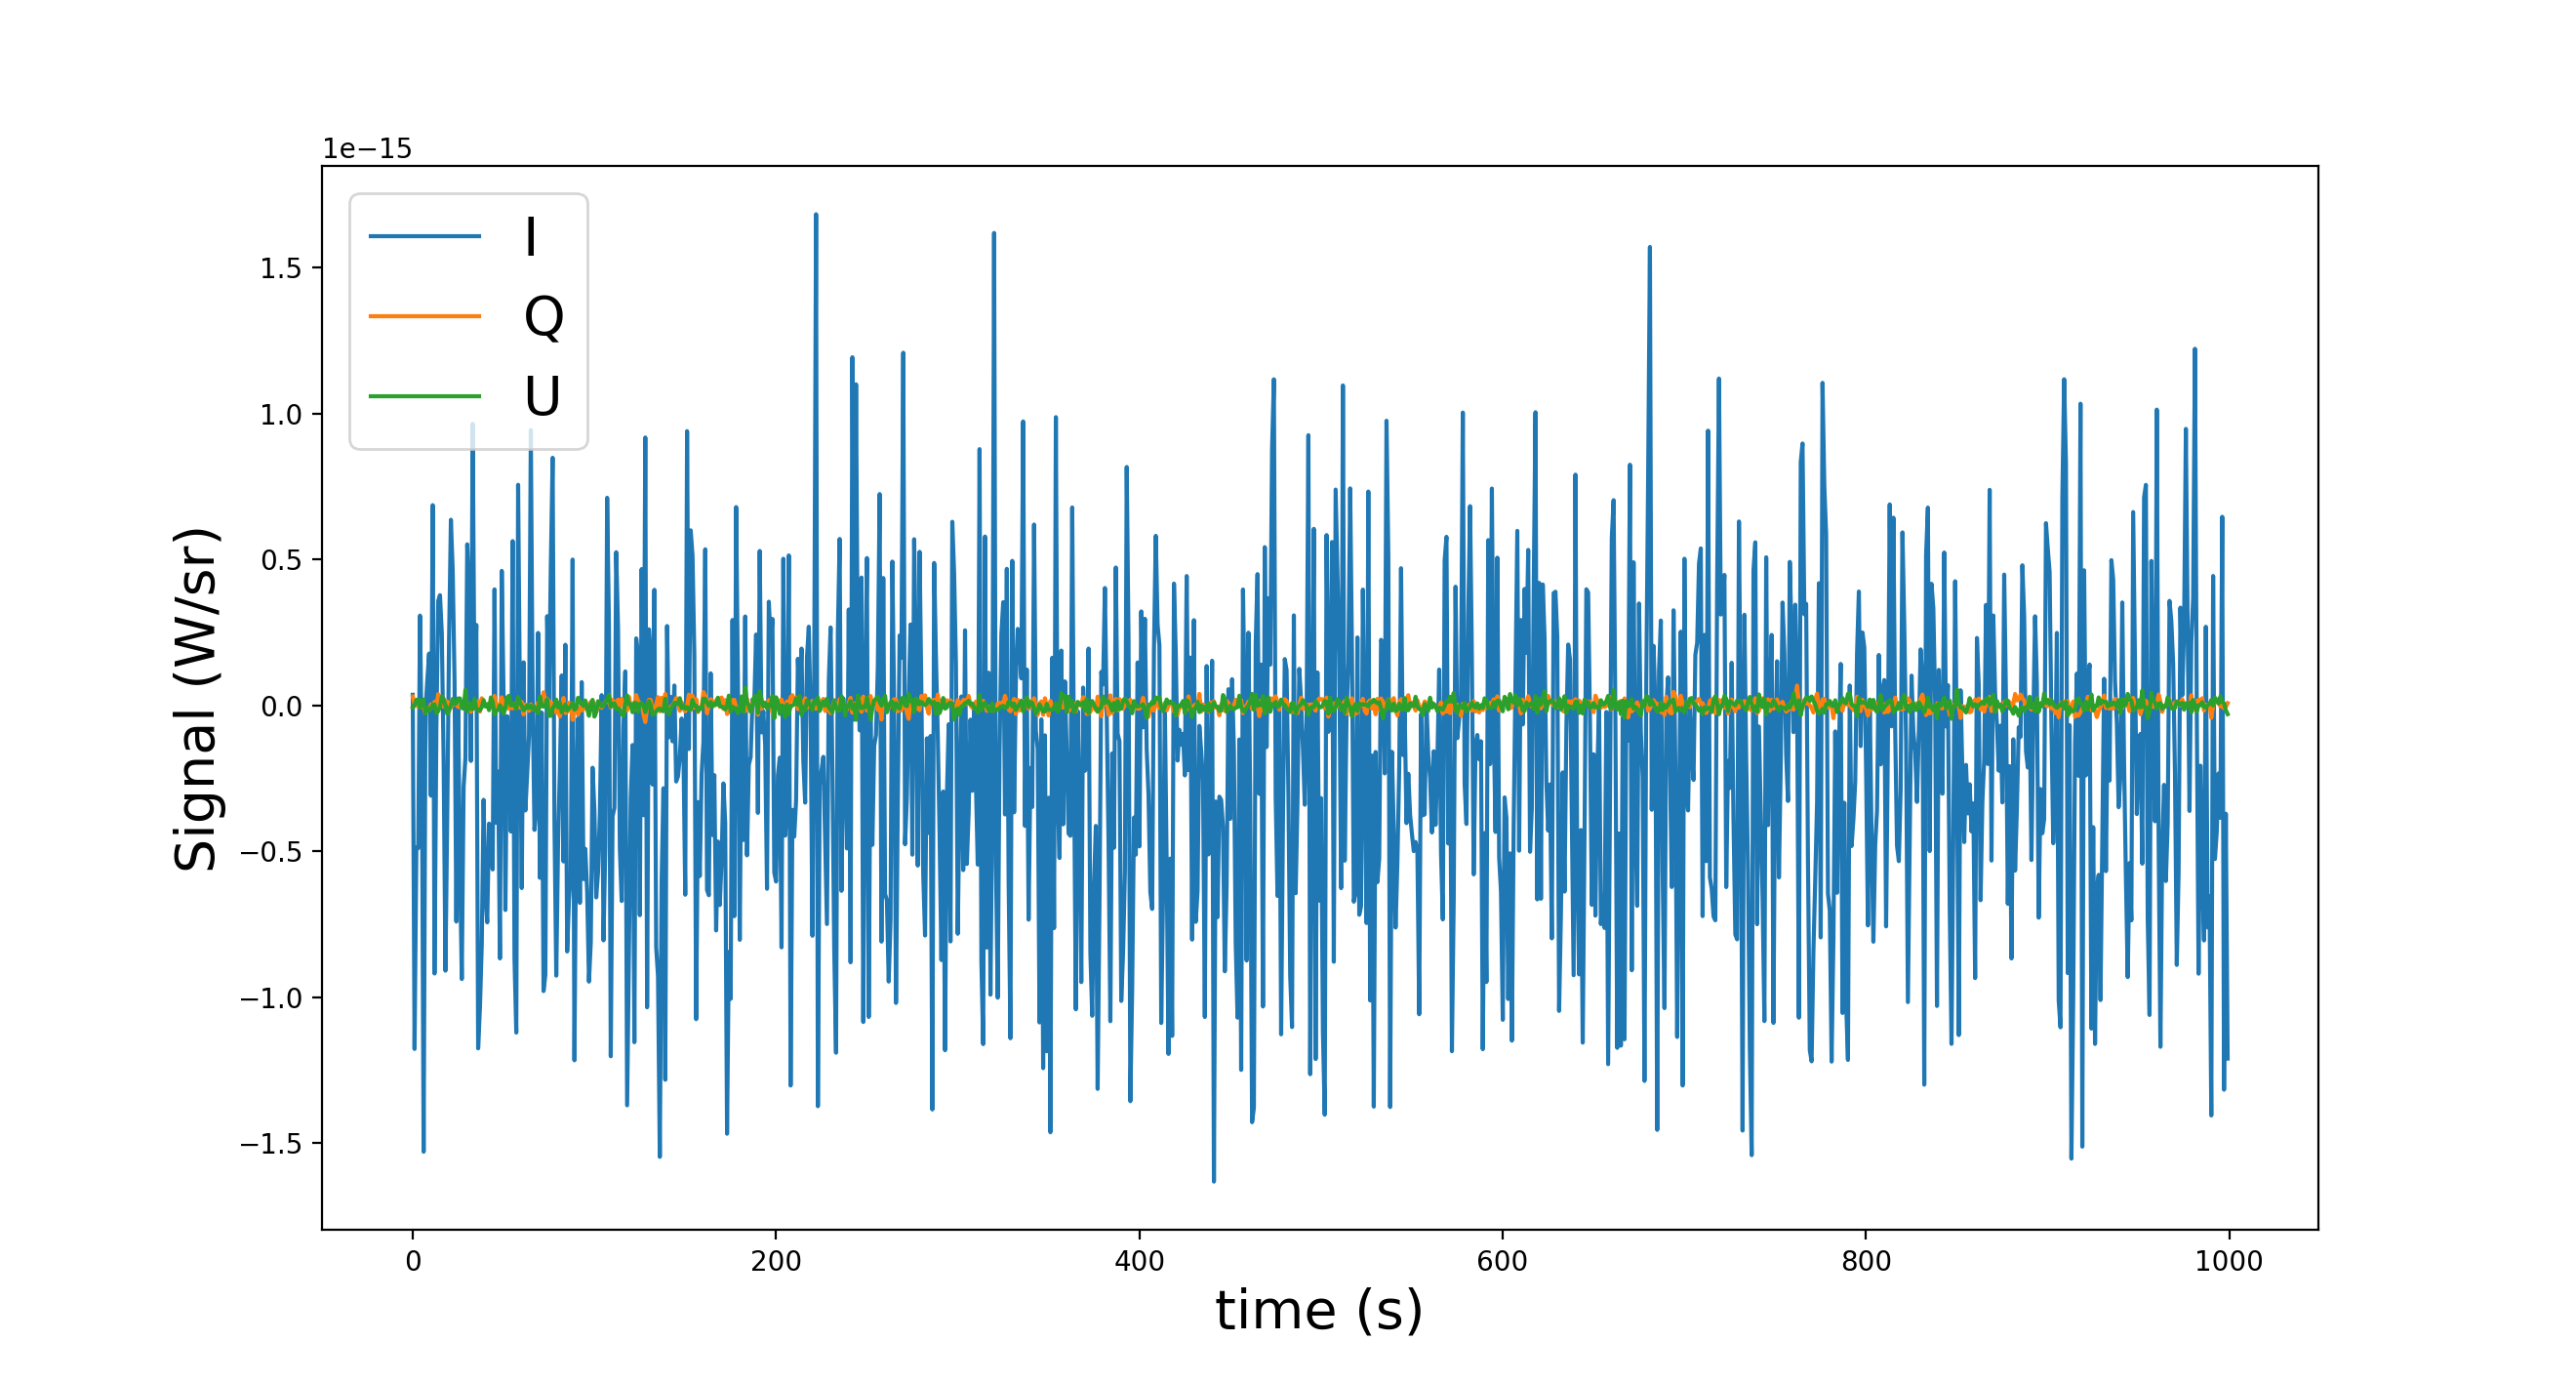
\includegraphics[width=1\textwidth]{TOD.png}
  \caption{TOD of I,Q and U obtained using the projection operator, this is an intermediate step before obtaining the full signal seen by the detector.}
  \label{fig:TOD}
\end{figure}


\section{Map making}

The code uses a maximum likelihood map making algorithm to go from TOD to map.
The TOD can be written as
\ba
\bm {d}=  \bm {{\cal H} m }+ \bm {n}
\ea
Assuming a gaussian noise with covariance $\bm{{\cal N}}$ we can write down the likelihood function of measuring $\bm{d}$ given $\bm{m}$
\ba
-2 \ln {\cal L} \propto ( \bm{d}- \bm {{\cal H} m })^{T} \bm{{\cal N}^{-1}}  (\bm{d}- \bm {{\cal H} m })
\ea
We can find the maximum likelihood solution of the system by taking the derivative with respect to $\bm{m}$
\ba
\frac{ \partial \ln {\cal L}}{ \partial \bm{m}} &=& -2  \bm {{\cal H} }^{T} \bm{{\cal N}^{-1}}  (\bm{d}- \bm {{\cal H }m  }) =0 \\
\bm {m}&=& ( \bm {{\cal H} }^{T} \bm{{\cal N}^{-1}} \bm {{\cal H }  })^{-1}    \bm {{\cal H} }^{T} \bm{{\cal N}^{-1}} \bm{d}
\ea
One choice is thus the noise covariance matrix, it should be as close as possible to the noise present on the data. There are two different noise covariance matrices that can be used in the code:

\begin{enumerate}
\item
${\it get\_diag\_invntt\_operator}$ which return a diagonal invariance noise covariance matrix taking into account detector noise and photon noise
\ba
{\cal N}^{-1}= (\sigma^{2}_{\rm det} + \sigma^{2}_{\gamma})^{-1} 
&=& = 2 T_{s} ({\rm NEP}^{2}_{\rm det} + {\rm NEP}^{2}_{\gamma})^{-1} 
\ea
Where $T_{s}$ is the sampling period in s.
We can rescale the noise per sample using an effective duration, this can be propagated to the noise covariance matrix in the following way
\ba
{\cal N}_{\rm eff}^{-1}=  {\cal N}^{-1}  \frac{ 365 \times 24 \times3600 \times N_{\rm yr} }{ N_{\rm sample} T_{s}}
\ea
\item
${\it get\_invntt\_operator}$ which return the full inverse covariance matrix and can include correlated noise in the time streams

\end{enumerate}


\section{Scene}

 Scene contains  routines to do rotation and  unit conversion  and to specify  the atmospheric properties.


\section{Input sky}

Once the frequency band of the instrument have been specified, we need to simulate the sky in each of the frequency band, for the moment I use $\it{create\_input\_cmb\_sky}$ that return a copy of I,Q,U for the 10 frequencies band.



\end{document}
